%%%%%%%% ICML 2019 EXAMPLE LATEX SUBMISSION FILE %%%%%%%%%%%%%%%%%

\documentclass{article}

% Recommended, but optional, packages for figures and better typesetting:
\usepackage{microtype}
\usepackage{graphicx}
\usepackage{subfigure}
\usepackage{booktabs} % for professional tables

% hyperref makes hyperlinks in the resulting PDF.
% If your build breaks (sometimes temporarily if a hyperlink spans a page)
% please comment out the following usepackage line and replace
% \usepackage{icml2019} with \usepackage[nohyperref]{icml2019} above.
\usepackage{hyperref}

% Attempt to make hyperref and algorithmic work together better:
\newcommand{\theHalgorithm}{\arabic{algorithm}}
\newcommand{\dds}{DDS}

%\usepackage[utf8]{inputenc} % allow utf-8 input
%\usepackage[T1]{fontenc}    % use 8-bit T1 fonts
%\usepackage{nicefrac}       % compact symbols for 1/2, etc.
%\usepackage[normalem]{ulem}

\usepackage[linesnumbered,ruled]{algorithm2e}
\usepackage{adjustbox}
\usepackage{mathtools}
% Use the following line for the initial blind version submitted for review:
\usepackage{icml2019}
\usepackage{wrapfig}

% If accepted, instead use the following line for the camera-ready submission:
%\usepackage[accepted]{icml2019}

% The \icmltitle you define below is probably too long as a header.
% Therefore, a short form for the running title is supplied here:
\icmltitlerunning{Optimizing Data Usage via Differentiable Rewards}
%\usepackage{times}
%usepackage{fullpage}
\usepackage{float}
\usepackage{graphicx}
\usepackage{amsmath}
%\usepackage[numbers,sort]{natbib}
%\usepackage[
%  pagebackref,
%  pageanchor=true,
%  plainpages=false,
%  pdfpagelabels,
%  bookmarks,
%  bookmarksnumbered,
%  colorlinks=true,
%  citecolor=blue,
%  menucolor=green,
%%pdfborder=0 0 0,  %removes outlines around hyper links in online display
%]{hyperref}
\usepackage{subfigure}
\usepackage{microtype}
\usepackage{url}
\usepackage{amsfonts}
\usepackage{amssymb}
\usepackage{amsthm}
\usepackage{mathrsfs}
\usepackage{tikz}
\usepackage{graphicx}
\usepackage{verbatim}
\usepackage{xcolor}
\usepackage{booktabs}
\usepackage{multirow}
\usepackage{todonotes}
\usepackage{footnote}
\usepackage{wrapfig}
\usepackage{blindtext}
\usepackage{caption}
\usepackage{mwe}
% \usepackage{algorithm}
\usepackage{algorithmic}

\makesavenoteenv{tabular}
\usepackage[toc,page]{appendix}
\usepackage{comment}

\newcommand{\cf}{\textit{c.f.}}
\newcommand{\eg}{\textit{e.g.}}
\newcommand{\ie}{\textit{i.e.}}
\newcommand{\etc}{\textit{etc.}}
\newcommand{\fix}{\marginpar{FIX}}
\newcommand{\new}{\marginpar{NEW}}
\newcommand{\z}{\mathbf{z}}
\newcommand{\Z}{\mathbf{Z}}
\newcommand{\y}{\mathbf{y}}
\newcommand{\Y}{\mathbf{Y}}
\newcommand{\x}{\mathbf{x}}
\newcommand{\X}{\mathbf{X}}
\newcommand{\m}{\mathbf{m}}
\newcommand{\s}{\mathbf{s}}
\newcommand{\h}{\mathbf{h}}
\newcommand{\W}{\mathbf{W}}
\newcommand{\expected}[1]{\textbf{E}\left[ #1 \right]}
\newcommand{\variance}[1]{\textbf{Var}\left[ #1 \right]}
\newcommand{\covariance}[1]{\textbf{Cov}\left[ #1 \right]}
\newcommand{\vectornorm}[1]{\left\| #1 \right\|}
\newcommand{\expo}[1]{\exp{\left( #1 \right)}}
\newcommand{\ABS}[1]{\left| #1 \right|}
\newtheorem{theorem}{Theorem}
\newtheorem{proposition}{Proposition}
\newcommand{\defeq}{\mathrel{\stackrel{\makebox[0pt]{\mbox{\normalfont\tiny def}}}{=}}}

\newcommand{\enas}{ENAS}

\def\prerl{RL pretraining\xspace}
\def\as{active search\xspace}
\def\btheta{\vec{\theta}}
\def\bphi{\vec{h}}
\def\bphii{\vec{h}^{(n)}}
\def\ba{\vec{a}}
\def\bas{\vec{a}^{(k)}}
\def\bb{\vec{b}}
\def\bc{\vec{c}}
\def\bd{\vec{d}}
\def\be{\vec{e}}
\def\bbf{\vec{f}} % ugh, oh well
\def\bg{\vec{g}}
\def\bh{\vec{h}}
\def\bi{\vec{i}}
\def\bj{\vec{j}}
\def\bk{\vec{k}}
\def\bl{\vec{l}}
\def\bm{\vec{m}}
\def\bn{\vec{n}}
\def\bo{\vec{o}}
\def\bp{\vec{p}}
\def\bq{\vec{q}}
\def\br{\vec{r}}
\def\bs{\vec{s}}
\def\bsi{\vec{s}^{(n)}}
\def\bt{\vec{t}}
\def\bu{\vec{u}}
\def\bv{\vec{v}}
\def\bw{\vec{w}}
\def\bx{\vec{x}}
\def\by{\vec{y}}
\def\bz{\vec{z}}
\def\bxi{\bx^{(i)}}
\def\bysi{\by^{(i)*}}

\DeclareMathOperator*{\argmax}{argmax}
\DeclareMathOperator*{\argmin}{argmin}
\begin{document}

\twocolumn[
\icmltitle{Optimizing Data Usage via Differentiable Rewards}

% It is OKAY to include author information, even for blind
% submissions: the style file will automatically remove it for you
% unless you've provided the [accepted] option to the icml2019
% package.

% List of affiliations: The first argument should be a (short)
% identifier you will use later to specify author affiliations
% Academic affiliations should list Department, University, City, Region, Country
% Industry affiliations should list Company, City, Region, Country

% You can specify symbols, otherwise they are numbered in order.
% Ideally, you should not use this facility. Affiliations will be numbered
% in order of appearance and this is the preferred way.
\icmlsetsymbol{equal}{*}

\begin{icmlauthorlist}
\icmlauthor{Aeiau Zzzz}{equal,to}
\icmlauthor{Bauiu C.~Yyyy}{equal,to,goo}
\icmlauthor{Cieua Vvvvv}{goo}
\icmlauthor{Iaesut Saoeu}{ed}
\icmlauthor{Fiuea Rrrr}{to}
\icmlauthor{Tateu H.~Yasehe}{ed,to,goo}
\icmlauthor{Aaoeu Iasoh}{goo}
\icmlauthor{Buiui Eueu}{ed}
\icmlauthor{Aeuia Zzzz}{ed}
\icmlauthor{Bieea C.~Yyyy}{to,goo}
\icmlauthor{Teoau Xxxx}{ed}
\icmlauthor{Eee Pppp}{ed}
\end{icmlauthorlist}

\icmlaffiliation{to}{Department of Computation, University of Torontoland, Torontoland, Canada}
\icmlaffiliation{goo}{Googol ShallowMind, New London, Michigan, USA}
\icmlaffiliation{ed}{School of Computation, University of Edenborrow, Edenborrow, United Kingdom}

\icmlcorrespondingauthor{Cieua Vvvvv}{c.vvvvv@googol.com}
\icmlcorrespondingauthor{Eee Pppp}{ep@eden.co.uk}

% You may provide any keywords that you
% find helpful for describing your paper; these are used to populate
% the "keywords" metadata in the PDF but will not be shown in the document
\icmlkeywords{Machine Learning, ICML}

\vskip 0.3in
]

% this must go after the closing bracket ] following \twocolumn[ ...

% This command actually creates the footnote in the first column
% listing the affiliations and the copyright notice.
% The command takes one argument, which is text to display at the start of the footnote.
% The \icmlEqualContribution command is standard text for equal contribution.
% Remove it (just {}) if you do not need this facility.

%\printAffiliationsAndNotice{}  % leave blank if no need to mention equal contribution
\printAffiliationsAndNotice{\icmlEqualContribution} % otherwise use the standard text.


\begin{abstract}
To acquire a new skill, humans learn better and faster if a private tutor, based on their current knowledge level, inform them whether they should pay extra attention to a practice problem. Similarly, a machine learning model could potentially be trained more efficiently with instructions on the importance of a training data that dynamically ``adapt'' to its current learning state. Meanwhile, identifying the optimal and dynamic importance measure for training any model is a challenging problem, because in order to quantify the effect of a modification to training data importance at a given time during the training, one needs to wait for the whole training process to finish. 
In this paper, we propose Differentiable Adaptive Weighting~(\dds), a novel method for selecting high-quality training data. We formulate the training data importance weight as a parameterized function that is updated along with the main model being trained. The formulation allows direct differentiation to optimize the adaptive data weight, and we show that the derived update rule is equivalent to Reinforcement Learning update with an intuitive reward function. Without significant computing overhead, \dds~delivers strong and consistent improvements on two modalities. Specifically, on multilingual machine translation, \dds~can dynamically identify which related languages are helpful to improve the translation of another language, leading to consistent improvements over a strong heuristic data selection baseline. On image classification tasks with CIFAR-10 and ImageNet, and with different ranges of data, \dds~can also optimize the importance of different training instances throughout training, leading to consistent improvements over the baselines in all settings.\footnote{We will release the code after the paper get accepted.}

\end{abstract}
\section{\label{sec:intro} Introduction}
To train a deep learning model, the standard method is to perform uniform stochastic gradient update steps on batches of training data, although the data provided might have many differences in quality, structure or domain properties. Many prior work strive to improve model performance by designing better data selection strategies. Research on data filtering has found that removing noisy data, or selecting in-domain or structurally similar data can lead to large improvements in model performance while potentially reducing the training time~\citep{jiang-zhai-2007-instance,wang-etal-2017-instance,axelrod2011domain,foster-etal-2010-discriminative,moore2010intelligent}. More broadly, data selection can help transfer learning and domain adaptation, where good strategies on using data from a resource rich domain/task can significantly improve the target domain/task we are interested in. For example, while training on data from related high-resource languages is an effective approach for improve the model performance on low-resource languages, identifying the good related languages to use is crucial for a competitive model~\citep{TCS}. 
%Another related line of research is curriculum learning, which improves the model performance by presenting the model easy examples first and then moving towards harder examples~\citep{cl_bengio}.      

There are several challenges shared by existing approaches on training data selection: first, the design of data filtering/selection criterion relies on domain-specific knowledge and hand-picked heuristics; second, most data usage strategies are predefined before the training start and thus is deterministic throughout the training process. 
%Although curriculum learning generally applies different data order at different training steps, the curriculum is a predefined ordering which cannot adapt to the model once training starts. 
Given the existing challenges, we ask the question: ``can we design an algorithm that automatically and efficiently learn the optimal training data that can adapt to the training state of any given learning model?''

We propose a general algorithmic framework for automatic data selection that works by optimizing a data weighting function throughout the training process. We formulate the training objective of the model itself as a weighted sum of the \textit{training} loss using a scoring function. We then optimize this scoring function so that the learned model parameters minimize the loss on the \textit{development} set. The optimization of adaptive data weight can be framed as a Reinforcement Learning problem, where we provide an intuitive reward function: given a model state, training data that has similar gradients with the dev data gets higher reward. Then we directly derive the update rule from the mathematical formulation and show that the gradient of the data weighting is equivalent to the proposed reward function. We name this method ``Differentiable Adaptive Weighting~(\dds)'', because the update rule allows us to directly optimize the data scoring function using back-propagation.

We demonstrate two concrete instantiations of the \dds~framework, one for a more general case of image classification, and the other for a more specific use case on neural machine translation~(NMT). For image classification, we test the algorithm on both CIFAR-10 and ImageNet. For NMT, we focus on a multilingual setting, where we select data from a multilingual corpus to improve the performance on a particular language. 
\section{\label{sec:method} Differentiable Data Selection}
%\gn{Here the explanation is definining a bunch of variables without explaining how they are actually used in equations. This makes things at the beginning seem quite vague and it's hard to tell exactly what you're doing. I'd follow the more standard ML practice of defining variables at the same time that you define the equations that use them. For example, shortly after (or before) you define the variables that are used in the scoring network, define what function the scoring network calculates. I think the previous version of the paper was quite good at doing this, so maybe go back and look at that and do something similar?}

\subsection{\label{sec:dds_motivation}Risk, Training, and Development Sets}
%\gn{I suggested some more descriptive section titles. Please take a look.}

Commonly in machine learning, we seek to find the parameters $\theta^*$ that minimize the \emph{risk} $J(\theta,P)$, the expected value of a loss function $\ell(x, y; \theta)$, where $\langle x, y \rangle$ are pairs of inputs and associated labels sampled from a particular distribution $P(X, Y)$:
\begin{equation}
  \label{eqn:generic_optim}
  \begin{aligned}
   & \theta^* = \argmin_\theta J(\theta, P)
    ~~~\text{where}~~~ \\
   & J(\theta, P) = \mathbb{E}_{x, y \sim P(X, Y)} [\ell(x, y; \theta)]
  \end{aligned}
\end{equation}

Ideally, we would like the risk $J(\cdot)$ to be minimized over the data distribution that our system sees at test time, ie.~$P_{\text{test}}(X,Y)$.
Unfortunately, this distribution is unknown at training time, so instead we collect a training set $\mathcal{D}_\text{train} = \{(x_i, y_i): i = 1, ..., N_\text{train}\}$ with distribution $P_\text{train}(X, Y) = \text{Uniform}(\mathcal{D}_\text{train})$, and minimize the \emph{empirical risk} by taking $\langle x, y \rangle \sim P_\text{train}(X, Y)$.
Since we need a sufficiently large training set $\mathcal{D}_\text{train}$ to train a good model, it is hard to ensure that $P_\text{train}(X, Y) \approx P_{\text{test}}(X, Y)$. In fact, we often accept that training data comes from a different distribution than test data.
The discrepancy between $P_\text{train}(X, Y)$ and $P_\text{test}(X, Y)$ manifests itself in the form of problems such as overfitting~\citep{overfit_random_examples,dropout}, covariate shift~\citep{shimodaira2000improving}, and label shift~\citep{lipton2018detecting}.

However, unlike the large training set, we can collect a relatively small development set $\mathcal{D}_\text{dev}= \{(x_i, y_i): i = 1, ..., N_\text{dev}\}$ with distribution $P_{\text{dev}}(X, Y)$ which is much closer to $P_{\text{test}}(X, Y)$\footnote{As is standard in machine learning experiments, we make sure that $\mathcal{D}_\text{dev}$ has no overlap with $\mathcal{D}_\text{train}$ or $\mathcal{D}_\text{test}$. Details of how we construct the $\mathcal{D}_\text{dev}$ can be found in Appendix \ref{app:nmt_hparam} and \ref{app:image_hparam}.}.
Since $\mathcal{D}_\text{dev}$ is a better approximation of our test-time scenario\footnote{For example, in Section \ref{sec:nmt_method} we would like to use training data from many different languages to improve the performance of a particular low-resource language. Here we can gather a small set of $\mathcal{D}_\text{dev}$ from the low resource language, even if we can’t gather a large training set in the language. Moreover, in a domain adaptation setting we can obtain a small dev set in the target domain, or in a setting of training on noisy data we can often obtain a small clean dev set.}, we can use $\mathcal{D}_\text{dev}$ to get reliable feedback to learn to better utilize our training data from $\mathcal{D}_\text{train}$. In particular, we propose to train a \emph{scorer} network, parameterized by $\psi$, to provide guidance on training data usage to minimize $J(\theta, \mathcal{D}_\text{dev})$ .


%\subsection{\label{sec:dds_motivation}Notation}
%We use $\theta$, $\psi$ to denote the parameters of the main model being trained and the scorer network respectively. $\mathcal{D}_\text{train}$, $\mathcal{D}_\text{dev}$ represent the train and development datasets. $\langle x, y \rangle$ 
%%\paul{you are not really using the fact that $x$ and $y$ are different things so I suggest you say "$z=(x, y)$ represents a sample" and then use $z$ instead of $x,y$ in the rest of the exposition} 
%represents a pair of data instance, and $X, Y$ represents the support of their corresponding distributions. The loss function to optimize is $\ell(\cdot)$ \gn{define this in equations}, and the risk $J(\cdot)$ \gn{define this in equations} represents the expected value of the loss function over a particular data distribution.

\subsection{\label{sec:efficient_reward} Reinforcement Learning for Optimizing Data Usage}
We propose to optimize the scorer's parameters $\psi$ in an RL setting.
%so that it can provide feedback about the effect of an example on the model's performance on the dev set, most existing work relies on an RL setting~\citep{rl_nmt,learn_to_teach,learn_active_learn}.
Our \emph{environment} is the model state $\theta$ and an example $\langle x, y \rangle$. Our RL \emph{agent} is the scorer network $\psi$, which optimizes the data usage for the current model state. The agent's~\emph{reward} on picking an example approximates the dev set performance of the resulting model after the model is updated on this example.
%\gn{One thing that is not clear throughout the description below is whether the action of the scorer network is to \emph{sample} an example or \emph{weight} an already-sampled example. In this section, it seems like it's the latter, but then in the next section it suddenly switches to talking about sampling. This probably needs to be made clear.}

% To optimize the scorer's parameters $\psi$ so that it can provide feedback about the effect of an example on the model's performance on the dev set, most existing work relies on an RL setting~\citep{rl_nmt,learn_to_teach,learn_active_learn}. Generally, the \emph{environment} is the model state $\theta$ and the data $\langle x, y \rangle$. The \emph{agent} to optimize is the scorer network $\psi$, which provides the value of the data for a given model state. The \emph{reward} for training on a given data is generally measured using change in dev set performance. 

% However, the above RL framework is difficult to implement in practice for two reasons. First, to make the agent, or scorer network, adaptive to the model state, it is generally formulated as a function of features from both the model training state and the data~\citep{rl_nmt,learn_to_teach,mentornet}. However, the feature design is a complicated problem in itself and might involve heuristic estimates. Second, the reward being the dev set performance change makes optimization difficult. Formally, the reward can be written as $\Delta J_{\text{dev}}(x, y) = J(\theta_t, \mathcal{D}_\text{dev}) - J(\theta_{t-1}, \mathcal{D}_\text{dev})$, where $\theta_t$ is the new model parameter after updating $\theta_{t-1}$ using the training data $(x, y)$. If we want to get clear credit assignment of a single training data pair $(x, y)$, its reward $\Delta J_{\text{dev}}(x, y)$ would be very noisy, because in practice the dev set is relatively small. To reduce the variance in $\Delta J_{\text{dev}}(x, y)$, we need a large number of training pairs $(x, y) = \{(x_0, y_0), (x_1, y_1), ..., (x_i, y_i)\}$. These examples would all get assigned the same amount of reward, while they might have different level of actual influence on the final model performance.

Our scorer network is parameterized as a differentiable function that only takes as inputs the features of the example $\langle x, y \rangle$. Intuitively, it represents a distribution over the training data where more important data has a higher probability of being used, denoted $P(X, Y; \psi)$. Unlike prior methods which generally require complicated featurization of both the model state and the data as input to the RL agent~\citep{learn_to_teach,mentornet,learn_active_learn}, our formulation is much simpler and  generalizable to different tasks. Since our scorer network does not consider the model parameters $\theta_t$ as input, we update it iteratively with the model so that at training step $t$, $P(X, Y; \psi_t)$ provides an up-to-date data scoring feedback for a given $\theta_t$. %This design makes our scorer network task-agnostic %\gn{This is not entirely true, as the network needs to encode $\langle x, y\rangle$, and the method to do so is task specific. This is probably just a problem of wording, but we should try to be precise. Also, it's not clear what the alternative, non-task-agnostic method would be. If you're trying to draw a contrast to previous work, for example, it would be good to state it explicitly.}.

Although the above formulation is simpler and more general, it requires much more frequent updates to the scorer parameter $\psi$. Existing RL frameworks simply use the change in dev set risk as the regular reward signal, which makes the update expensive and unstable~\citep{learn_to_teach,rl_nmt}. Therefore, we propose a novel reward function as an approximation to $\Delta J_{\text{dev}}(x, y)$ to quantify the effect of the training example $\langle x, y \rangle$. Inspired by \citet{cos_sim} (which uses gradient similarity between two tasks to measure the adaptation effect between them, we use the agreement between the model gradient on data $\langle x, y \rangle$ and the gradient on the dev set to approximate the effect of $\langle x, y \rangle$ on dev set performance. This reward simply implies that we prefer data that moves $\theta$ in the direction that minimizes the dev set risk: 
\begin{equation}
    \label{eqn:reward_fn}
\begin{align}
     R(x, y) & = \Delta J_{\text{dev}}(x, y) \\
    & \approx \nabla_\theta \ell(x, y; \theta_{t-1})^\top \cdot \nabla_\theta J(\theta_t, \mathcal{D}_\text{dev}) 
\end{align}
\end{equation}

According to the REINFORCE algorithm~\citep{reinforce}, the update rule for $\psi$ is thus
\begin{equation}
\label{eqn:psi_update}
\begin{aligned}
    & \psi_{t+1} \leftarrow  \psi_t + \\
    &  \underbrace{\nabla_\theta \ell(x, y; \theta_{t-1}) \cdot \nabla_\theta J(\theta_t, \mathcal{D}_\text{dev})}_{\mathclap{R(x, y)}} \nabla_\psi \text{log}(P(X, Y;\psi))
\end{aligned}
\end{equation}
%where $\eta$ is the learning rate for the scorer parameter $\psi$. 
The update rule for the model is simply
\begin{align}
    \label{eqn:theta_update}
    \theta_t \leftarrow \theta_{t-1} - \nabla_\theta J(\theta_{t-1}, P(X, Y;\psi))
\end{align}
%where $\alpha$ is the learning rate for the model. 
For simplicity of notation, we omit the learning rate term. Full derivation can be found in Appendix \ref{app:grad_of_optimizers}. By alternating between Eqn.~\ref{eqn:theta_update} and Eqn.~\ref{eqn:psi_update}, we can iteratively update $\theta$ using the guidance from the scorer network, and update $\psi$ to optimize the scorer using feedback from the model.  

Our formulation of scorer network as $P(X, Y; \psi)$ has several advantages. First, it provides the flexibility that we can either sample a training instance or equivalently scale the update from the training instance based on its score. Specifically, we provide an algorithm under the \dds~framework for multilingual NMT~(see Sec. \ref{sec:nmt_method}), where the former is more efficient, and another more general algorithm for image classification~(see Sec. \ref{sec:image_method}), where the latter choice is natural. Second, it allows easy integration of prior knowledge of the data, which is shown to be effective in Sec. \ref{sec:experiment}. 

\subsection{\label{sec:diff_data_selection}Deriving Rewards through Direct Differentiation}
In this section, we show that the update for the scorer network in Eqn.~\ref{eqn:psi_update} can be approximately derived as the solution of a bi-level optimization problem~\citep{bilevel_optim}, which has been applied to many different lines of research~\citep{hyper_grad,darts,learn_reweight}. 

Under our framework, the scorer samples the data by $\langle x, y \rangle \sim P(X, Y; \psi)$, and $\psi$ will be chosen so that $\theta^*$ that optimizes $J(\theta, P(X, Y;\psi))$ will approximately minimize $J(\theta, P_\text{dev}(X,Y))$: 
\begin{equation}
  \label{eqn:psi_theta_argmin}
  \begin{aligned}
   & \psi^* = \argmin_\psi
  J(\theta^*(\psi), \mathcal{D}_\text{dev}) 
    ~\text{where}~ \\
   & \theta^*(\psi) = \argmin_\theta \mathbb{E}_{x, y \sim P(X, Y; \psi)} \left[ \ell(x, y; \theta) \right]
  \end{aligned}
\end{equation}

The connection between $\psi$ and $\theta$ in Eqn. \ref{eqn:psi_theta_argmin} shows that $J(\theta_t, \mathcal{D}_\text{dev})$ is differentiable with respect to $\psi$. Now we can approximately compute the gradient $\nabla_\psi J(\theta_t, \mathcal{D}_\text{dev})$ as follows:
%\gn{The labels of the following equation are outside of the right margin. Try to fix this (I tried using negative ``hspace'' but unfortunately that  didn't work.)}:
%\begin{equation}
%  \label{eqn:two_step_update}
%   \small
%  \begin{aligned}
%   & \nabla_\psi J(\theta_t, \mathcal{D}_\text{dev})\\
%    &= \nabla_{\theta_t} J(\theta_t, \mathcal{D}_\text{dev})^\top \cdot \nabla_\psi \theta_t(\psi) ~~\quad\quad\quad\quad\%quad\quad\quad\quad \text{(chain rule)} \\
%      &= \nabla_{\theta_t} J(\theta_t, \mathcal{D}_\text{dev})^\top \cdot \nabla_\psi \left( \theta_{t-1} - \nabla_\theta J(%\theta_{t-1}, \psi) \right) \quad \text{(substitute $\theta_t$ from Eqn~\ref{eqn:theta_update})} \\
%      &\approx -\nabla_{\theta_t} J(\theta_t, \mathcal{D}_\text{dev})^\top \cdot \nabla_\psi  \left( \nabla_\theta J(\theta_%{t-1}, \psi) \right) ~~\quad\quad\quad \text{(assume $\nabla_\psi \theta_{t-1} \approx 0$)} \\
%      &= -\nabla_\psi \mathbb{E}_{x, y \sim P(X, Y; \psi)} \left[\nabla_\theta J(\theta_t, \mathcal{D}_\text{dev})^\top \%cdot \nabla_\theta \ell(x, y; \theta_{t-1} )\right] \\
%    &= -\mathbb{E}_{x, y \sim P(X, Y; \psi)} \left[\left( \nabla_\theta J(\theta_t, \mathcal{D}_\text{dev})^\top \cdot \%nabla_\theta \ell(x, y; \theta_{t-1} ) \right) \cdot \nabla_\psi \log{P(x, y; \psi)} \right]
%  \end{aligned}
%\end{equation}

\begin{equation}
  \label{eqn:two_step_update}
  \begin{aligned}
   & \nabla_\psi J(\theta_t, \mathcal{D}_\text{dev})\\
   & \quad\quad\quad\quad \text{apply chain rule:} \\
    &= \nabla_{\theta_t} J(\theta_t, \mathcal{D}_\text{dev})^\top \cdot \nabla_\psi \theta_t(\psi) \\
    & \quad\quad\quad\quad  \text{substitute $\theta_t$ from Eqn~\ref{eqn:theta_update}:} \\
      &= \nabla_{\theta_t} J(\theta_t, \mathcal{D}_\text{dev})^\top \cdot \nabla_\psi \left( \theta_{t-1} - \nabla_\theta J(\theta_{t-1}, \psi) \right)  \\
      & \quad\quad\quad\quad  \text{assume $\nabla_\psi \theta_{t-1} \approx 0$:} \\
      &\approx -\nabla_{\theta_t} J(\theta_t, \mathcal{D}_\text{dev})^\top \cdot \nabla_\psi  \left( \nabla_\theta J(\theta_{t-1}, \psi) \right) \\
      &= -\nabla_\psi \mathbb{E}_{x, y \sim P(X, Y; \psi)} \left[\nabla_\theta J(\theta_t, \mathcal{D}_\text{dev})^\top \cdot \nabla_\theta \ell(x, y; \theta_{t-1} )\right] \\
    &= -\mathbb{E}_{x, y \sim P(X, Y; \psi)} \left[\left( \nabla_\theta J(\theta_t, \mathcal{D}_\text{dev})^\top \cdot \nabla_\theta \ell(x, y; \theta_{t-1} ) \right) \\
    & \quad\quad\quad\quad\quad\quad\quad\quad\quad\quad\quad\quad\quad\quad\quad \cdot \nabla_\psi \log{P(x, y; \psi)} \Big]
  \end{aligned}
\end{equation}
Here, we make a Markov assumption\footnote{Our use of the Markov assumption is based on its use and empirical success in previous work on bi-level optimization, such as Hyper Gradient Descent (Baydin et al. 2017) and many others. Intuitively, this assumption indicates in the previous step $\psi_{t-1}$ is already updated regards to $\theta_{t-1}$, so the effect of $\psi$ on $\theta_{t-1}$ is likely to be minimal.} that $\nabla_\psi \theta_{t-1} \approx 0$, assuming that at step $t$, given $\theta_{t-1}$ we do not care about how the values of $\psi$ from previous steps led to $\theta_{t-1}$. Eqn.~\ref{eqn:two_step_update} leads to a rule to update $\psi$ using gradient descent, which is exactly the same as the RL update rule in Eqn.~\ref{eqn:psi_update}.
%\gn{This is exactly the same as equation 3. We can just reference equation 3 instead of rewriting it here. This will also save a lot of space, we can basically remove the rest of this paragraph (including the name of the method.)}:
%\begin{equation}
%  \label{eqn:psi_update_rule}
%   \small
%  \begin{aligned}
%    \psi_{t+1} 
%      &\leftarrow \psi_t + \eta \left(\nabla_\theta J(\theta_t, \mathcal{D}_\text{dev})^\top \cdot \nabla_\theta \ell(x, y; \theta_{t-1} ) \right) \cdot \nabla_\psi \log{P(x, y; \psi)},
%  \end{aligned}
%\end{equation}
%where $\eta$ is the learning rate for $\psi$, which is a hyper-parameter. Now we can see that our derived update rule Eqn. \ref{eqn:psi_update_rule} matches the update rule for the scorer network in Eqn. \ref{eqn:psi_update}. Since the update rule for our scorer network approximately follows a direct differentiation to optimize $\psi$, we name it Differentiable Adaptive Teaching~(\dds) \gn{If you don't delete this part, make sure to fix the name here.}.

%To implement Eqn~\ref{eqn:psi_update} we need two approximations. First, in practice the size of $\mathcal{D}_\text{train}$ is usually too large for exact calculation of the gradient $\nabla_\theta$. To overcome this difficulty, we adopt an importance sampling strategy, which can be implemented in two ways: (1) We can sample a subset of $\mathcal{D}_{\text{train}}$ with a uniform proposal distribution $\hat{x}, \hat{y} \sim \text{Uniform}(\mathcal{D}_\text{train})$, then scale the probabilities in Eqn~\ref{eqn:psi_theta_argmin} by $p(\hat{x}, \hat{y}; \psi)$ over only this subset of data. (2) We can similarly sample a subset of $\mathcal{D}_{\text{train}}$ uniformly, but then take a Monte-Carlo estimate of this quantity by further sub-sampling the data according to $p(\hat{x}, \hat{y}; \psi)$. Second, the exact gradient for $\psi$ depends on the optimization algorithm that we use for $\theta$, and we discuss details of the derivations in Appendix \ref{app:grad_of_optimizers}.
\subsection{Additional Derivation Details and Clarifications}
Note that our derivation above does not take into the account that we might use different optimizing algorithms, such as SGD or Adam~\citep{adam}, to update $\theta$. We provide detailed derivations for several popular optimization algorithms in Appendix \ref{app:grad_of_optimizers}.  In practice, we use cosine distance instead of dot product to measure the gradient alignment between training and dev data, because cosine distance has smaller variance and thus makes the scorer update more stable.    

One potential concern with our approach is that because we optimize $\psi_t$ directly on the dev set using $J(\theta_t, \mathcal{D}_\text{dev})$, we may risk indirectly overfitting model parameters $\theta_t$ by selecting a small subset of data that is overly specialized.
However we do not observe this problem in practice, and posit that this because (1) the influence of $\psi_t$ on the final model parameters $\theta_t$ is quite indirect, and acts as a ``bottleneck'' which has similarly proven useful for preventing overfitting in neural models \cite{grezl2007probabilistic}, and (2) because the actual implementations of \dds~(which we further discuss in Section \ref{sec:formualtion}) only samples a subset of data from $\mathcal{D}_\text{train}$ at each optimization step, further limiting expressivity.


\section{\label{sec:formualtion}Concrete Instantiations of DDS}

%\gn{I made a few changes here, please tell me if you think they aren't warranted: (1) I moved this sentence into this section from the end of the previous section, (2) I removed the mention of ``Momentum'' and ``Adam'' in the below sentence, as it seemed to hurt generality, (3) I tried to note that image classification is ``generic'' and multilingual NMT is ``specific'', so as a general ML paper people can see that this is both broadly applicable and customizable.}
We now turn to discuss two concrete instantiations of DDS that we use in our experiments: a more generic example of classification, which should be applicable to a wide variety of tasks, and a specialized application to the task of multilingual NMT, which should serve as an example of how DDS can be adapted to the needs of specific applications.

%\gn{In the following, for further generality, (1) can we turn ``Image Classification'' into just ``Classification''? (2) can we remove any other details that hurt the generality of the approach such as specific mention of ``Momentum'' or ``Adam'', mentioning that the classification model is a CNN, etc.? These can be moved to the experiments.}

\subsection{\label{sec:image_method}Formulation for Classification}

%\begin{wraptable}{l}{8cm}
    \vspace{-0.2cm}
\begin{center}
\resizebox{!}{3.1cm}{
\begin{algorithm}[H]
\SetAlgoLined
\DontPrintSemicolon
\SetKwInOut{Input}{Input}
\SetKwInOut{Output}{Output}
\SetCommentSty{itshape}
\SetKwComment{Comment}{$\triangleright$\ }{}
\Input{$\mathcal{D}_\text{train}$, $\mathcal{D}_\text{dev}$}
\Output{Optimal parameters $\theta^*$}
 Initializer $\theta_0$ and $\psi_0$
 
 \For{$t = 1$~\textbf{\emph{to}}~$\text{num\_train\_steps}$}{
    Sample $B$ training data points $x_i, y_i \sim \text{Uniform}(\mathcal{D}_\text{train})$
    
    Sample $B$ validation data points $x'_i, y'_i \sim \text{Uniform}(\mathcal{D}_\text{dev})$
  
    \Comment{Optimize $\theta$}
    Update $\theta_t \leftarrow \text{GradientUpdate}\Big(\theta_{t-1}, \sum_{i=1}^{B} p(x_i, y_i; \psi_{t-1}) \nabla_\theta \ell(x_i, y_i; \theta_{t-1}) \Big)$
    \label{alg:grad_update_model}
    
    \Comment{Evaluate $\theta_t$ on $\mathcal{D}_\text{dev}$}
    Let $d_\theta \leftarrow \frac{1}{B} \sum_{j=1}^{B} \nabla_\theta \ell(x'_j, y'_j; \theta_t)$
  
    \Comment{Optimize $\psi$}
    Let $d_\psi \leftarrow \frac{1}{B} \sum_{i=1}^{B} \left[ \Big( d_\theta^\top \cdot \nabla_\theta \ell(x_i, y_i; \theta_{t-1}) \Big) \cdot \nabla_\psi \log{p(x_i, y_i; \psi)} \right]$
    \label{alg:require_per_example_grad}
    
    Update $\psi_t \leftarrow \text{GradientUpdate}(\psi_{t-1}, d_\psi)$
    \label{alg:grad_update_p}
  }
  \caption{\label{alg:image_classification_dds}Training a classification model with \dds.}
\end{algorithm}
}
\end{center}
    \vspace{-0.2cm}

%\end{wraptable}
Algorithm~\ref{alg:image_classification_dds} presents the pseudo code for the training process on classification tasks, using the notations introduced in Section~\ref{sec:method}. 
The main  classification model is parameterized by $\theta$. The scorer $p(X, Y; \psi)$ is an identical network with the main model, but with independent weights, \ie~$p(X, Y; \psi)$ does not share weights with $\theta$. For each example $x_i$ in a minibatch uniformly sampled from $\mathcal{D}_\text{train}$, this \dds~model outputs a scalar from the data $x_i$. All scalars are passed through a softmax function to compute the relative probabilities of the examples in the minibatch, and their gradients are scaled accordingly when applied to $\theta$. Note that our actual formulation of $p(X, Y; \psi)$ does \textit{not} depend on $Y$, but we keep $Y$ in the notation for consistency with the formulation of the \dds~framework. Note that we have two gradient update steps, one for the model parameter $\theta_t$ in Line~\ref{alg:grad_update_model} and the other for the \dds~scorer parameter $\psi$ in Line~\ref{alg:grad_update_p}. For the model parameter update, we can simply use any of the standard optimization update rule. For the scorer $\psi$, we use the update rule derived in Section \ref{sec:diff_data_selection}.

\paragraph{Per-Example Gradient.} As seen from Line~\ref{alg:require_per_example_grad} of Algorithm~\ref{alg:image_classification_dds}, as well as from Eqn.~\ref{eqn:momentum_update_for_psi}, \dds~requires us to compute $\nabla_\theta \ell(x_i, y_i; \theta_{t-1})$, \ie~the gradient for each example in a batch of training data. This operation is very slow and memory intensive, especially when the batch size is large, \eg~our experiments on ImageNet use a batch size of $4096$ (see~Section~\ref{sec:experiment}). Therefore, we propose an efficient approximation of this per-example gradient computation via the first-order Taylor expansion of $\ell(x_i, y_i; \theta_{t-1})$. In particular, for any vector $v \in \mathbb{R}^{\ABS{\theta}}$, with sufficiently small $\epsilon > 0$, we have:
    \vspace{-0.15cm}
\begin{equation}
  \label{eqn:taylor_dot_product}
  \small
  \begin{aligned}
    v^\top \cdot \nabla_\theta \ell(x_i, y_i; \theta_{t-1})
    \approx
    \frac{1}{\epsilon}
    \left(
      \ell\big( x_i, y_i; \theta_{t-1} + \epsilon v \big) -
      \ell\big( x_i, y_i; \theta_{t-1} \big)
    \right),
  \end{aligned}
\end{equation}
    %\vspace{-0.1cm}
Eqn~\ref{eqn:taylor_dot_product} can be implemented by keeping a shadow version of parameters $\theta_{t-1}$, caching training loss $\ell(x_i, y_i; \theta_{t-1})$, and computing the new loss with $\theta_{t-1} + \epsilon v$. Here, $v$ is $d_\theta$ as in Line~\ref{alg:require_per_example_grad} of Algorithm~\ref{alg:image_classification_dds}.

\subsection{\label{sec:nmt_method}Formulation for Multilingual NMT}

In this section, we demonstrate an application of DDS to multilingual models for NMT, specifically applied to improving accuracy on low-resource languages (LRL)~\citep{nmt_transfer,rapid_adapt_nmt,johnson_nmt}.
In this setting, we assume that we have a particular LRL $S$ that we would like to translate into target language $T$, and we additionally have a multilingual corpus $\mathcal{D}_{\text{train}}$ that has parallel data between $n$ source languages $(S_1, S_2, ..., S_n)$ and target language $T$.
We would like to pick parallel data from any of the source languages to the target language to improve translation of a particular LRL $S$, so we assume that $\mathcal{D}_{\text{dev}}$ exclusively consists of parallel data between $S$ and $T$.
As a result, DDS will attempt to select data from $\mathcal{D}_{\text{train}}$ that improve accuracy on $S$-to-$T$ translation as represented by $\mathcal{D}_{\text{dev}}$.
% We then train a parameterized distribution $p(x, y;\psi)$ with a support over $\mathcal{D}_{\text{train}}$, such that selecting training data according to this distribution leads to the optimal NMT model $\theta^*$ on the language $S$. 
%That is, $\psi$ satisfies the following condition
%\begin{equation}
%  \label{eqn:nmt_argmin}
%  \begin{aligned}
%    \arg\min_\psi
%    \sum_{x_i, y_i \in S\text{-}Y} \ell_{\text{dev}}(x_i, y_i; \theta^*)
%    ~~~\text{where}~~~
%    \theta^* = \arg\min_\theta \mathbb{E}_{x_i,y_i \sim p(X, Y;\psi)}\left[ \ell_{\text{train}}(x_i, y_i; \theta) \right]
%  \end{aligned}
%\end{equation}
%\begin{wraptable}{l}{8cm}
    %\vspace{-0.3cm}
    \vspace{-0.2cm}
\begin{center}
\resizebox{!}{3.3cm}{
\begin{algorithm}[H]
\SetAlgoLined
\DontPrintSemicolon
\SetKwInOut{Input}{Input}
\SetKwInOut{Output}{Output}
\SetCommentSty{itshape}
\SetKwComment{Comment}{$\triangleright$\ }{}
%\KwResult{Write here the result }

\Input{$\mathcal{D}_{\text{train}}$; K: number of data to train the NMT model before updating $\psi$; 
E: number of updates for $\psi$; 
$\alpha_1$,$\alpha_2$: discount factors for the gradient}

\Output{The converged NMT model $\theta^*$}

  Initialize $\psi_0$, $\theta_0$
  
  \Comment{Initialize the gradient of each source language}
  $grad[S_i] \leftarrow 0$ \textbf{for} \textit{i in n}
  %\For{ i in n}{
  %
  %  $grad[S_i] \leftarrow 0$
  %  
  %}
 
  \While{$\theta$ not converged}{
    %\Comment{Sample training data according to $\psi$}
    $X, Y \leftarrow \text{load\_data}(\psi, \mathcal{D}_{\text{train}}, K)$  \label{alg:load_nmt}
  
    \Comment{Train the NMT model}
    \For{ $x_i, y$ in $X, Y$}{
      $\theta_t \leftarrow \text{GradientUpdate}\left( \theta_{t-1}, \nabla_{\theta_{t-1}} \ell(x_i, y; \theta_{t-1}) \right)$
        
      $grad[S_i] \leftarrow \alpha_1 \times \text{grad}[S_i] + \alpha_2 \times \nabla_{\theta_{t-1}} \ell(x_i, y; \theta_{t-1})$
    }
  
    \Comment{Optimize $\psi$}
    \For{ iter in E}{
      
      sample $B$ data pairs from $\mathcal{D}_{\text{train}}$
      
      $d_\psi \leftarrow \frac{1}{B} \sum_{j=1}^B \sum_{i=1}^n \left[ \text{grad}[S_i]^\top \text{grad}[S] \cdot \nabla_{\psi_{t-1}} \text{log}\left( p\left( S_i|y_j;\psi_{t-1} \right) \right) \right]$
       
      $\psi_t \leftarrow \text{GradientUpdate}(\psi_{t-1}, d_{\psi_{t-1}})$ 
    }
  }
  \caption{\label{alg:nmt_dds}Training multilingual NMT with DDS.}
\end{algorithm}
}
\end{center}
    \vspace{-0.2cm}
%\end{wraptable} 

To make training more efficient and stable in this setting, we make three simple modifications of the main framework in Section \ref{sec:diff_data_selection} that take advantage of the problem structure of multilingual NMT.
First, instead of directly modeling $p(X,Y;\psi)$, we assume a uniform distribution over the target sentence $Y$, %($p(Y)$)
and only parameterize the conditional distribution of which source language sentence to pick given the target sentence: $p(X|y;\psi)$. This design follows the formulation of Target Conditioned Sampling~(TCS~\citep{TCS}), an existing state-of-the-art data selection method with a similar structure, but models the distribution $p(X|y)$ using heuristics.
Second, we only update $\psi$ after updating the NMT model for a fixed number of steps.
Third, we sample the data according to $p(X|y;\psi)$ to get a Monte Carlo estimate of the objective in Equation \ref{eqn:psi_theta_argmin}.
This can significantly reduce the training time compared to using all data.
The pseudo code of the training process is in Algorithm \ref{alg:nmt_dds}.

%Note that in Line \ref{alg:load_nmt} of Algorithm \ref{alg:nmt_dds}, we load $K$ training data according to $p(\psi)$. Since we formulate $p(\psi)$ as $p(S_i|y;\psi)$, the data loading procedure is the same as the TCS algorithm~\citep{TCS}: for each of the $K$ target sentences, we calculate a distribution over its source languages according to $p(S_i|y;\psi)$, and then sample the corresponding source sentences based on this distribution.

 


\begin{table*}[t]
  \caption{\label{tab:results}Results for image classification accuracy (left) and multilingual MT BLEU (right). For MT, the statistical significance is indicated with $*$ (p $<$ 0.005) and $\dagger$ (p $<$ 0.0001). \dds~ outperforms the best baseline in all settings. For both image classification and NMT, \dds~performs better than other intelligent data selection methods.}
  \vspace{0.2cm}
   \begin{minipage}{.59\linewidth}
    \resizebox{\textwidth}{!}{
      \begin{tabular}{lcccc}
        \toprule
        \multirow{2}{*}{\textbf{Methods}}
        & \multicolumn{2}{c}{CIFAR-10 (WRN-28-$k$)} & \multicolumn{2}{c}{ImageNet (ResNet-50)} \\
        \cmidrule(lr){2-3} \cmidrule(lr){4-5}
        & 4K, $k=2$ & Full, $k=10$ & 10\% & Full \\
        \midrule
        Uniform &
        82.60$\pm$0.17 &
        95.55$\pm$0.15 & 
        56.36/79.45 &
        76.51/93.20 \\
        SPCL &
        81.09$\pm$0.22 &
        93.66$\pm$0.12 & 
        - &
        - \\
        BatchWeight &
        79.61$\pm$0.50 &
        94.11$\pm$0.18 & 
        - &
        - \\
        MentorNet &
        83.11$\pm$0.62 &
        94.92$\pm$0.34 & 
        - &
        - \\
        \midrule
        \dds     &
        83.63$\pm$ 0.29 &
        96.31$\pm$ 0.13 &
        \textbf{56.81}/\textbf{79.51} &
        \textbf{77.23}/\textbf{93.57} \\
         retrained \dds     &
        \textbf{85.56}$\pm$\textbf{0.20} &
        \textbf{97.91}$\pm$\textbf{0.12} &
        - &
        - \\       
        \bottomrule
      \end{tabular}
      }
      \end{minipage}
      \hfill
  \begin{minipage}{.4\linewidth}
    \resizebox{\textwidth}{!}{
      \begin{tabular}{l|cccc}
        \toprule
        \textbf{Methods} & \textbf{aze} & \textbf{bel} & \textbf{glg} & \textbf{slk} \\
        \midrule
        Uniform & 10.31 & 17.21 & 26.05 & 27.44 \\
        SPCL & 9.07 & 16.99 & 23.64 & 21.44 \\
        Related & 10.34 & 15.31 & 27.41 & 25.92 \\
        TCS     & 11.18 & 16.97 & 27.28 & 27.72 \\
        \midrule
        \dds     & 10.74 & 17.24 & 27.32 & $\mathbf{28.20^*}$ \\
        TCS+\dds & $\mathbf{11.84^*}$ & $\mathbf{17.74^\dagger}$ & \textbf{27.78} & 27.74 \\
        \bottomrule
      \end{tabular}
      }
      \end{minipage}
\end{table*}

\section{\label{sec:experiment}Experiments}
%\gn{You need at least one sentence of lead-in here.}
We now discuss experimental results on both image classification, an instance of the general classification problem using \autoref{alg:image_classification_dds}, and multilingual NMT using \autoref{alg:nmt_dds}.

\subsection{\label{exp:settings}Experimental Settings}

% \gn{One reviewer asked how the development sets are created. It seems like this needs to be mentioned here?} \cw{i added a footnote in the method section and included the details in appendix?} \gn{I found that now. Looks OK.}

\noindent \textbf{Data.} We apply our method on established benchmarks for image classification and multilingual NMT.
For image classification, we use CIFAR-10~\citep{cifar10} and ImageNet~\citep{imagenet}. For each dataset, we consider two settings: a reduced setting where only roughly 10\% of the training labels are used, and a full setting, where all labels are used. Specifically, the reduced setting for CIFAR-10 uses the first $4000$ examples in the training set, and with ImageNet, the reduced setting uses the first $102$ TFRecord shards as pre-processed by~\citet{imagenet_generalize_better}. We use the size of $224 \times 224$ for ImageNet.

For multilingual NMT, we use the 58-language-to-English TED dataset~\citep{ted_pretrain_emb}. 
Following prior work~\citep{ted_pretrain_emb,rapid_adapt_nmt,sde}, we evaluate translation from four low-resource languages~(LRL) Azerbaijani~(\texttt{aze}), Belarusian~(\texttt{bel}), Galician~(\texttt{glg}), and Slovak~(\texttt{slk}) to English, where each is paired with a similar high-resource language Turkish~(\texttt{tur}), Russian~(\texttt{rus}), Portugese~(\texttt{por}), and Czech~(\texttt{ces}) (details in \autoref{app:nmt_data}).
We combine data from all 8 languages, and use \dds~to optimize data selection for each LRL.

To update the scorer, we construct $\mathcal{D}_\text{dev}$ so that it does not overlap with $\mathcal{D}_\text{test}$. For image classification, we hold out $10\%$ of the training data as $\mathcal{D}_\text{dev}$; while for multilingual NMT, we simply use the dev set of the LRL as $\mathcal{D}_\text{dev}$.

\noindent \textbf{Models and Training Details.}
For image classification, on CIFAR-10, we use the pre-activation WideResNet-28~\citep{wide_res_net}, with width factor $k=2$ for the reduced setting and $k=10$ for the normal setting. For ImageNet, we use the post-activation ResNet-50~\citep{res_net}. 
%The batch sizes for CIFAR-10 and for ImageNet are $128$ and $4096$, running for 200K steps and 40K steps, respectively. 
%We use the standard Momentum update for the \dds~model parameter $\theta$, and the derived Momentum update rule in Section~\autoref{sec:grad_of_optimizers} for the \dds~distribution parameter $\psi$, both with the momentum rate of $0.9$.
These implementations reproduce the numbers reported in the literature~\citep{wide_res_net,res_net,resnext}, and additional details can be found in \autoref{app:image_hparam}.

For NMT, we use a standard LSTM-based attentional baseline \citep{attention}, which is similar to previous models used in low-resource scenarios on this dataset~\citep{rapid_adapt_nmt,sde} and others~\citep{lownmt19} due to its relative stability compared to other options such as the Transformer \citep{vaswani2017attention}. Accuracy is measured using BLEU score \citep{bleu}.
More experiment details are noted in \autoref{app:nmt_hparam}.

\noindent \textbf{Baselines and Our Methods.}
For both image classification and multi-lingual NMT, we compare the following data selection methods. \textbf{Uniform}: data is selected uniformly from all of the data that we have available, as is standard in training models. \textbf{SPCL}~\citep{spcl}: a curriculum learning method that dynamically updates the curriculum to focus more on the ``easy'' training examples based on model loss. \textbf{\dds}: our proposed method.
%\begin{itemize}
%\item \textbf{Uniform}: data is selected uniformly from all of the data that we have available, as is standard in training models. 
%\item \textbf{SPCL}~\citep{spcl}: a curriculum learning method that dynamically updates the curriculum to focus more on the ``easy'' training examples based on model loss.
%\item \textbf{\dds}: our proposed method.
%\end{itemize}

For image classification, we compare with several additional methods designed for filtering noisy data on CIFAR-10, where we simply consider the dev set as the clean data. \textbf{BatchWeight}~\citep{learn_reweight}: a method that scales example training loss in a batch with a locally optimized weight vector using a small set of clean data. \textbf{MentorNet}~\citep{mentornet}: a curriculum learning method that trains a mentor network to select clean data based on features from both the data and the main model.
%\begin{itemize}
%\item \textbf{BatchWeight}~\citep{learn_reweight}: a method that scales example training loss in a batch with a locally optimized weight vector using a small set of clean data. 
%\item  \textbf{MentorNet}~\citep{mentornet}: a curriculum learning method that trains a mentor network to select clean data based on features from both the data and the main model. 
%\end{itemize}


For machine translation, we also compare with two state-of-the-art heuristic methods for multi-lingual data selection. \textbf{Related}: data is selected uniformly from the target LRL and a linguistically related HRL \citep{rapid_adapt_nmt}. \textbf{TCS}: a recently proposed method of ``target conditioned sampling'', which uniformly chooses target sentences, then picks which source sentence to use based on heuristics such as word overlap \citep{TCS}. Note that both of these methods take advantage of structural properties of the multi-lingual NMT problem, and do not generalize to other problems such as classification. 
%\begin{itemize}
%\item \textbf{Related}: data is selected uniformly from the target LRL and a linguistically related HRL \citep{rapid_adapt_nmt}. 
%\item  \textbf{TCS}: a recently proposed method of ``target conditioned sampling'', which uniformly chooses target sentences, then picks which source sentence to use based on heuristics such as word overlap \citep{TCS}. Note that both of these methods take advantage of structural properties of the multi-lingual NMT problem, and do not generalize to other problems such as classification.
%\end{itemize}

%\gn{This is a little bit sudden to appear here directly in the experiments section. It might be good to mention this at the end of Section \ref{sec:efficient_reward} as a method to incorporate prior information? I think mentioning this there is actually a very good thing, as it adds to another thing that the proposed framework can do. If we mention it here, on the other hand, it seems a little bit like a hack that we added on at the last minute to make things work.}
\paragraph{DDS with Prior Knowledge} \dds~is a flexible framework to incorporate prior knowledge about the data using the scorer network, which can be especially important when the data has certain structural properties such as language or domain. We test such a setting of \dds~for both tasks.

For image classification, we use \textbf{retrained \dds}, where we first train a model and scorer network using the standard \dds~till convergence. The trained scorer network can be considered as a good prior over the data, so we use it to train the final model from scratch again using \dds. For multilingual NMT, we experiment with \textbf{TCS+\dds}, where we initialize the parameters of \dds~with the TCS heuristic, then continue training. 



% \noindent \textbf{Data Selection Baselines.} We compare our method against three strong baselines: 1) All: all 8 languages are used for training without any data selection; 2) Bi: we train on the combined datasets of each LRL and its related HRL, which is a special case of data selection that requires prior linguistic knowledge; 3) TCS~\citep{TCS}: the state-of-the-art data selection method for multilingual NMT. Given a target sentence, TCS conditionally samples a source sentence from the candidate languages based on simple heuristics such as vocabulary overlap.

%\gn{Just a comment: I'm not a huge fan of this because it seems a bit hacky, but if it's what was necessary to make things work this time then that's fair}. 
% We note that all these three tricks are not needed for our experiments on CIFAR-10, where the batch size is much smaller.

\subsection{Main Results}


%\begin{table}[t]
%  \captionof{table}{\label{tab:results}Results for image classification accuracy (left) and multilingual MT BLEU (right). For MT, the statistical significance is indicated with $*$ (p < 0.005) and $\dagger$ (p < 0.0001).}
%  \begin{minipage}{.575\linewidth}
%    \resizebox{\textwidth}{!}{
%      \begin{tabular}{lcccc}
%        \toprule
%        \multirow{2}{*}{\textbf{Methods}}
%        & \multicolumn{2}{c}{CIFAR-10 (WRN-28-$k$)} & \multicolumn{2}{c}{ImageNet (ResNet-50)} \\
%        \cmidrule(lr){2-3} \cmidrule(lr){4-5}
%        & 4K, $k=2$ & Full, $k=10$ & 10\% & Full \\
%        \midrule
%        Uniform &
%        82.60$\pm$0.17 &
%        95.55$\pm$0.15 & 
%        56.36/79.45 &
%        76.51/93.20 \\
%        SPCL &
%        81.09$\pm$0.22 &
%        93.66$\pm$0.12 & 
%        - &
%        - \\
%        BatchWeight &
%        79.61$\pm$0.50 &
%        94.11$\pm$0.18 & 
%        - &
%        - \\
%        MentorNet &
%        83.11$\pm$0.62 &
%        94.92$\pm$0.34 & 
%        - &
%        - \\
%        \midrule
%        \dds     &
%        83.63$\pm$ 0.29 &
%        96.31$\pm$ 0.13 &
%        \textbf{56.81}/\textbf{79.51} &
%        \textbf{77.23}/\textbf{93.57} \\
%         retrained \dds     &
%        \textbf{85.56}$\pm$\textbf{0.20} &
%        \textbf{97.91}$\pm$\textbf{0.12} &
%        - &
%        - \\       
%        \bottomrule
%      \end{tabular}
%    }
%  \end{minipage}
%  \begin{minipage}{.425\linewidth}
%    \resizebox{\textwidth}{!}{
%      \begin{tabular}{l|cccc}
%        \toprule
%        \textbf{Methods} & \textbf{aze} & \textbf{bel} & \textbf{glg} & \textbf{slk} \\
%        \midrule
%        Uniform & 10.31 & 17.21 & 26.05 & 27.44 \\
%        SPCL & 9.07 & 16.99 & 23.64 & 21.44 \\
%        Related & 10.34 & 15.31 & 27.41 & 25.92 \\
%        TCS     & 11.18 & 16.97 & 27.28 & 27.72 \\
%        \midrule
%        \dds     & 10.74 & 17.24 & 27.32 & $\mathbf{28.20^*}$ \\
%        TCS+\dds & $\mathbf{11.84^*}$ & $\mathbf{17.74^\dagger}$ & \textbf{27.78} & 27.74 \\
%        \bottomrule
%      \end{tabular}
%    }
%  \end{minipage}
%  \vspace{-4mm}
%\end{table}

% \begin{wraptable}{r}{0.6\textwidth}
% %\begin{adjustbox}{max width=0.7\textwidth}
% \vspace{-1cm}
% \resizebox{0.6\textwidth}{!}{
%   \begin{tabular}{llll}
%     \multicolumn{4}{c}{\textbf{CIFAR-10} ($\text{mean} \pm \text{std}$ over $10$ runs)} \\
%   \toprule
%     \textbf{Portion} &
%     \textbf{Model} &
%     \textbf{Baseline} &
%     \textbf{\\dds}
%     \\
%   \midrule
%     4K &
%     WideResNet-28-2 &
%     $82.60 \pm 0.17$ & % 6109331
%     $\mathbf{83.63 \pm 0.29}$ % 6109486
%     \\
%     Full &
%     WideResNet-28-10 &
%     $95.55 \pm 0.15$ &  % 6153155
%     $\mathbf{96.31 \pm 0.13}$  % 6170380
%     \\
%   \bottomrule
%     \\
%     \multicolumn{4}{c}{\textbf{ImageNet} ($\text{Top-1}/\text{Top-5}$)} \\
%     \toprule
%     \textbf{Portion} &
%     \textbf{Model} &
%     \textbf{Baseline} &
%     \textbf{\\dds}
%     \\
%   \midrule
%     10\%  & ResNet-50 &
%     $56.36 / 79.45$ & % 5267621/workUnits/118
%     $\mathbf{56.81 / 79.51}$   % 6020481/workUnits/18
%     \\  
%     Full & ResNet-50 &
%     $76.51 / 93.20$ & % https://arxiv.org/abs/1810.12890
%     $\mathbf{77.23 / 93.57}$ % 6800564/workUnits/39
%     \\
%     \bottomrule
%   \end{tabular}
% }
%   \captionof{table}{\label{tab:image_classification_results}Image classification accuracy. Higher is better.}
% %\end{adjustbox}
% %\end{center}
% \end{wraptable}

% \noindent \textbf{Results.} Results are presented in Table~\autoref{tab:image_classification_results}. As can be seen, \\dds~improves the performance of all tasks considered. The best improvement is for CIFAR-10 using 4K labels. We posit that this is because when the  
%\gn{The following explanation is pretty weak because increasing the degrees of freedom of the model was not even one of our original motivations. Is there any way we can at least say something about how it (might be?) reducing the weight on outliers or something like that?} In our intuitions, \\dds~provides an extra degree of freedom to train the models, namely the per-example scaling of gradients. This extra degree of freedom is well-utilized by the $p(\hat{x}, \hat{y}; \psi)$ distribution, leading to the improvements.


% \subsection{Multilingual NMT}
% 
% \noindent \textbf{Baselines.} We compare our method against three strong baselines: 1) All: all 8 languages are used for training without any data selection; 2) Bi: we train on the combined datasets of each LRL and its related HRL, which is a special case of data selection that requires prior linguistic knowledge; 3) TCS~\citep{TCS}: the state-of-the-art data selection method for multilingual NMT. Given a target sentence, TCS conditionally samples a source sentence from the candidate languages based on simple heuristics such as vocabulary overlap.
% 
% \noindent \textbf{Implementation.} Here we clarify several design choices for Algorithm \autoref{alg:nmt_\dds}. To model the distribution $p(S_i|y;\psi)$, we use a 2-layer feed-forward network with hidden size of 32. The input vector for the network is a vector of size of source languages $n$, representing which of the languages contain a corresponding source sentence for a given target sentence $y$. We use the standard Adam update rule with learning rate of 0.001 for the NMT model parameter $\theta$, and the derived Adam update rule from Section~\autoref{sec:grad_of_optimizers} with learning rate~0.0001 for the distribution parameter $\psi$. 
% 
% We test two different settings for using \dds for multilingual  NMT: 1) TCS+\dds: we pretrain the network with the heuristic distribution from TCS before the \dds training process
% %. K in Algorithm \autoref{alg:nmt_dds} is set to be 50,000; 
% 2) Uniform+DDS: we train the network for $\psi$ from scratch. %At the start of training, K is set to be 5,000 to encourage exploration; after updating $\psi$ for 5 times, we also set it to 50,000.
% We run all experiments with 3 different random seeds and pick the median for each method. Additional hyperparameters are listed in Appendix~\autoref{app:nmt_hparam}.
% 
% \noindent \textbf{Results.}
% \begin{wraptable}{l}{0.6\textwidth}
% \begin{center}
% \vspace{-0.5cm}
%     \begin{tabular}{l|cccc}
%     \toprule
%     \textbf{Model} & \textbf{aze} & \textbf{bel} & \textbf{glg} & \textbf{slk} \\
%     \midrule
%     All & 10.31 & 17.21 & 26.05 & 27.44 \\
%     Bi & 10.34 & 15.31 & 27.41 & 25.92 \\
%     TCS & 11.18 & 16.97 & 27.28 & 27.72 \\
%     \midrule
%     TCS+DDS & \textbf{11.84} & \textbf{17.74} & \textbf{27.78} & 27.74 \\
%     %Uniform & 9.54 & 14.75 & 25.11 & 26.30 \\
%     Uniform+DDS & 10.74 & 17.24 & 27.32 & \textbf{28.20} \\
%     \bottomrule
%     \end{tabular}
%      \captionof{table}{\label{tab:nmt_result}BLEU score. Higher is better.}
% \end{center}
% \vspace{-0.5cm}
% \end{wraptable}

The results of the baselines and our method are listed in \autoref{tab:results}.
First, comparing the standard baseline strategy of ``Uniform'' and the proposed method of ``\dds'' we can see that in all 8 settings \dds~improves over the uniform baseline. This is a strong indication of both the consistency of the improvements that \dds~can provide, and the generality -- it works well in two very different settings. Next, we find that \dds~outperforms SPCL by a large margin for both of the tasks, especially for multilingual NMT. This is probably because SPCL weighs the data only by their easiness, while ignoring their relevance to the dev set, which is especially important in settings where the data in the training set can have very different properties such as the different languages in multilingual NMT. 

\dds~also brings improvements over the state-of-the-art intelligent data utilization methods. For image classification, \dds~outperforms MentorNet and BatchWeight on CIFAR-10 in all settings. For NMT, in comparison to Related and TCS, vanilla \dds~performs favorably with respect to these state-of-the-art data selection baselines, outperforming each in 3 out of the 4 settings (with exceptions of slightly underperforming Related on \texttt{glg} and TCS on \texttt{aze}).
In addition, we see that incorporating prior knowledge into the scorer network leads to further improvements. For image classification, retrained \dds~can significantly improve over regular \dds, leading to the new state-of-the-art result on the CIFAR-10 dataset. For mulitlingual NMT, TCS+\dds~achieves the best performance in three out of four cases (with the exception of \texttt{slk}, where vanilla \dds~already outperformed TCS).\footnote{Significance tests~\citep{significance_nmt} find significant gains over the baseline for \texttt{aze}, \texttt{slk}, and \texttt{bel}. For \texttt{glg}, \dds~without heuristics performs as well as the TCS baseline.}

\dds~does not incur much computational overhead. For image classification and multilingual NMT respectively, the training time is about $1.5\times$ and $2\times$ the regular training time without \dds. This contrasts favorably to previous methods that learn to select data using reinforcement learning. For example, in the IMDB movie review experiment in  \citet{learn_what_data_learn}, the data agent is trained for 200 episode, where each episode uses around 40\% of the whole dataset, requiring 80x more training time than a single training run. 
%\footnote{The code for multilingual NMT is not optimized, so its training time could be reduced further}.
%\section{\label{sec:analysis} Analysis}
%In this section, we perform an analysis of exactly how DDS is learning, and what kind of data it is learning to select.

\begin{wrapfigure}{R}{0.3\textwidth}
  \vspace{-10mm}
  \begin{center}
    \includegraphics[width=0.3\textwidth]{figs/cifar10_dds.eps}
  \end{center}
  \vspace{-4mm}
  \caption{\label{fig:dds_distribution}Class distributions of CIFAR-10 4K.}
  \vspace{-8mm}
\end{wrapfigure}

\subsection{Analysis of Image Classification}
 Prior work on heuristic based data selection has found that the model performs better if we feed higher quality data towards the end of training~\citep{dynamic_data_selection_nmt} or finetune the model with more relevant data~\citep{dynamic}. Here we verify this observation by analyzing the learned importance weight at the end of training for the image classification task. Figure \ref{fig:dds_distribution}, we show that at the end of training, the \dds learns to balance the class distribution, which is originally unbalanced due to the dataset creation. In Figure \ref{fig:dds_score}, we show that at the end of training, \dds assigns higher probabilities to images with clearer class content from ImageNet. These results show that \dds learns to focus on higher quality data towards the end of training.  

\begin{figure}
    \centering
    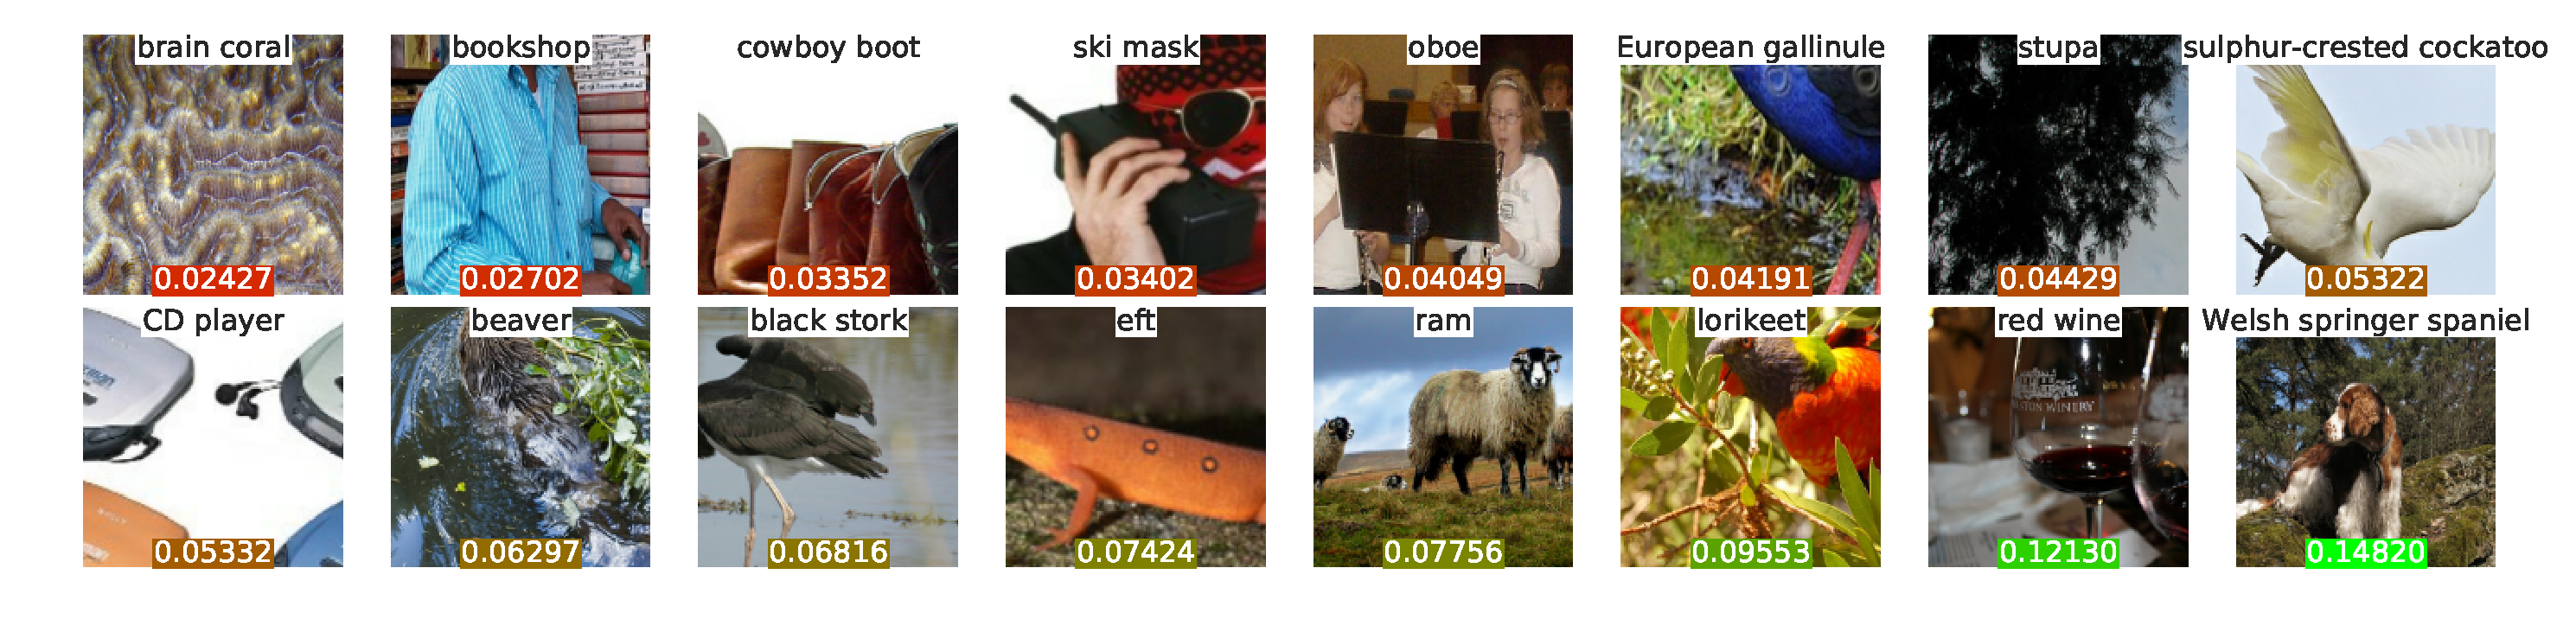
\includegraphics[width=\textwidth]{figs/imagenet_dds.eps}
  \caption{\label{fig:dds_score} Example images from the ImageNet and their weights assigned by \dds. }
\end{figure}

\subsection{Analysis of Multilingual NMT}
Next, we focus on multilingual NMT, where the choice of data directly corresponds to picking a language, which has an intuitive interpretation. Since \dds adapts the data weights dynamically to the model throughout training, here we analyze how the learned weights change throughout training.
%\begin{center}
%  \includegraphics[width=0.245\columnwidth]{figs/aze_devppl_plot.eps}
%  \includegraphics[width=0.23\columnwidth]{figs/bel_devppl_plot.eps}
%  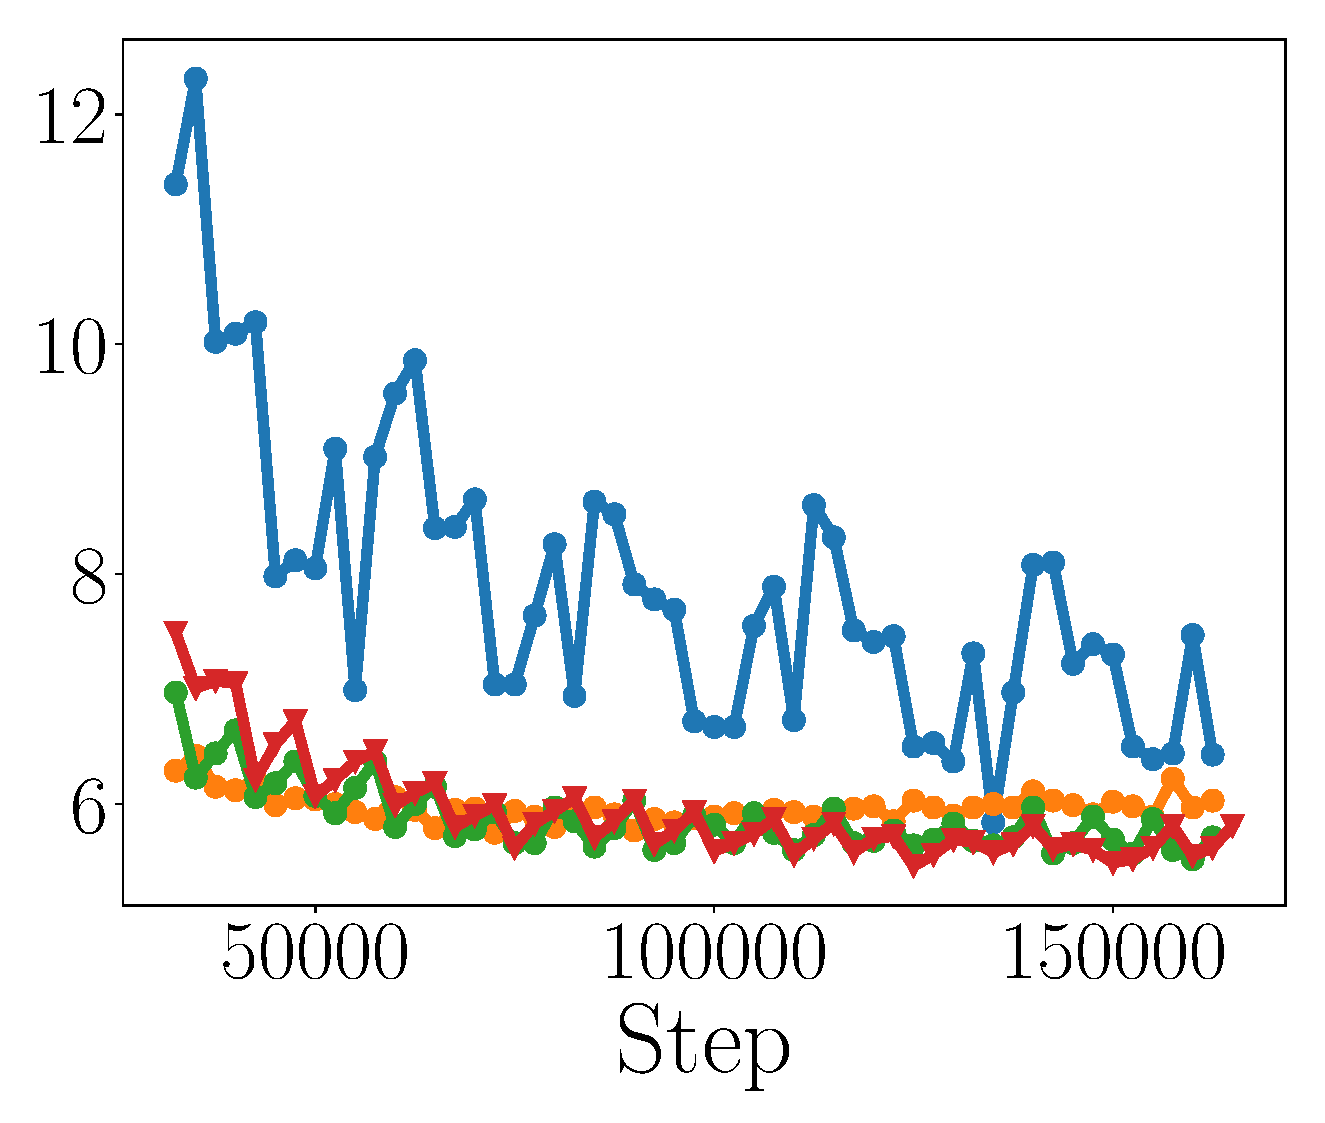
\includegraphics[width=0.23\columnwidth]{figs/glg_devppl_plot.eps}
%  \includegraphics[width=0.23\columnwidth]{figs/slk_devppl_plot.eps}
%  \captionof{figure}{\label{fig:nmt_converge}Development set perplexity vs. training steps. \textit{From left to right}: \texttt{aze}, \texttt{bel}, \texttt{glg}, \texttt{slk}.}
%\end{center}
%\paragraph{Training Curves.} First, we plot the dev set perplexity for three training methods, TCS, DDS, and TCS+DDS over the course of training in Figure \ref{fig:nmt_converge}.%
%\footnote{We did not plot ``Uniform'' here because it takes a far larger number of training steps to converge due to its uniform sampling of eight different languages, and thus is not visible on the same scale.}
%From the results, we can see that while DDS starts out with a higher perplexity than the TCS heuristics (which a-priori calculates the most appropriate language to be using based on surface statistics), it quickly catches up and surpasses TCS on all 4 languages.
%In addition, when initialized with the TCS heuristic, DDS starts at a relatively good perplexity and converges even faster.

\begin{center}
  \includegraphics[width=0.22\columnwidth]{figs/aze_hs_probs_plot.eps}
  \includegraphics[width=0.22\columnwidth]{figs/bel_hs_probs_plot.eps}
  \includegraphics[width=0.22\columnwidth]{figs/glg_hs_probs_plot.eps}
  \includegraphics[width=0.29\columnwidth]{figs/slk_hs_probs_plot.eps}
  \captionof{figure}{\label{fig:nmt_distrib_hs}Language usage for TCS$+$DDS by training step. \textit{From left to right}: \texttt{aze}, \texttt{bel}, \texttt{glg}, \texttt{slk}.}
\end{center}

%\paragraph{Learned Language Distributions.}
We plot the probability distribution of the four HRLs (because they have more data and thus larger impact on training) over the course of training.  Figure \ref{fig:nmt_distrib_hs} shows the change of language distribution for TCS+DDS. Since TCS selects the language with the largest vocabulary overlap with the LRL, the distribution is initialized to focus on the most related HRL. For all four LRLs, the percentage of their most related HRL starts to decrease as training continues. For \texttt{aze}, DDS quickly comes back to using its most related HRL. However, for \texttt{bel}, DDS continues the trend of using all four languages. This shows that DDS is able to maximize the benefits of the multilingual data by having a more balanced usage of all languages. 
%For gig and slk, DDS learns to mainly use both por and ces, their corresponding HRL.

\vspace{-0.2cm}
\begin{center}
  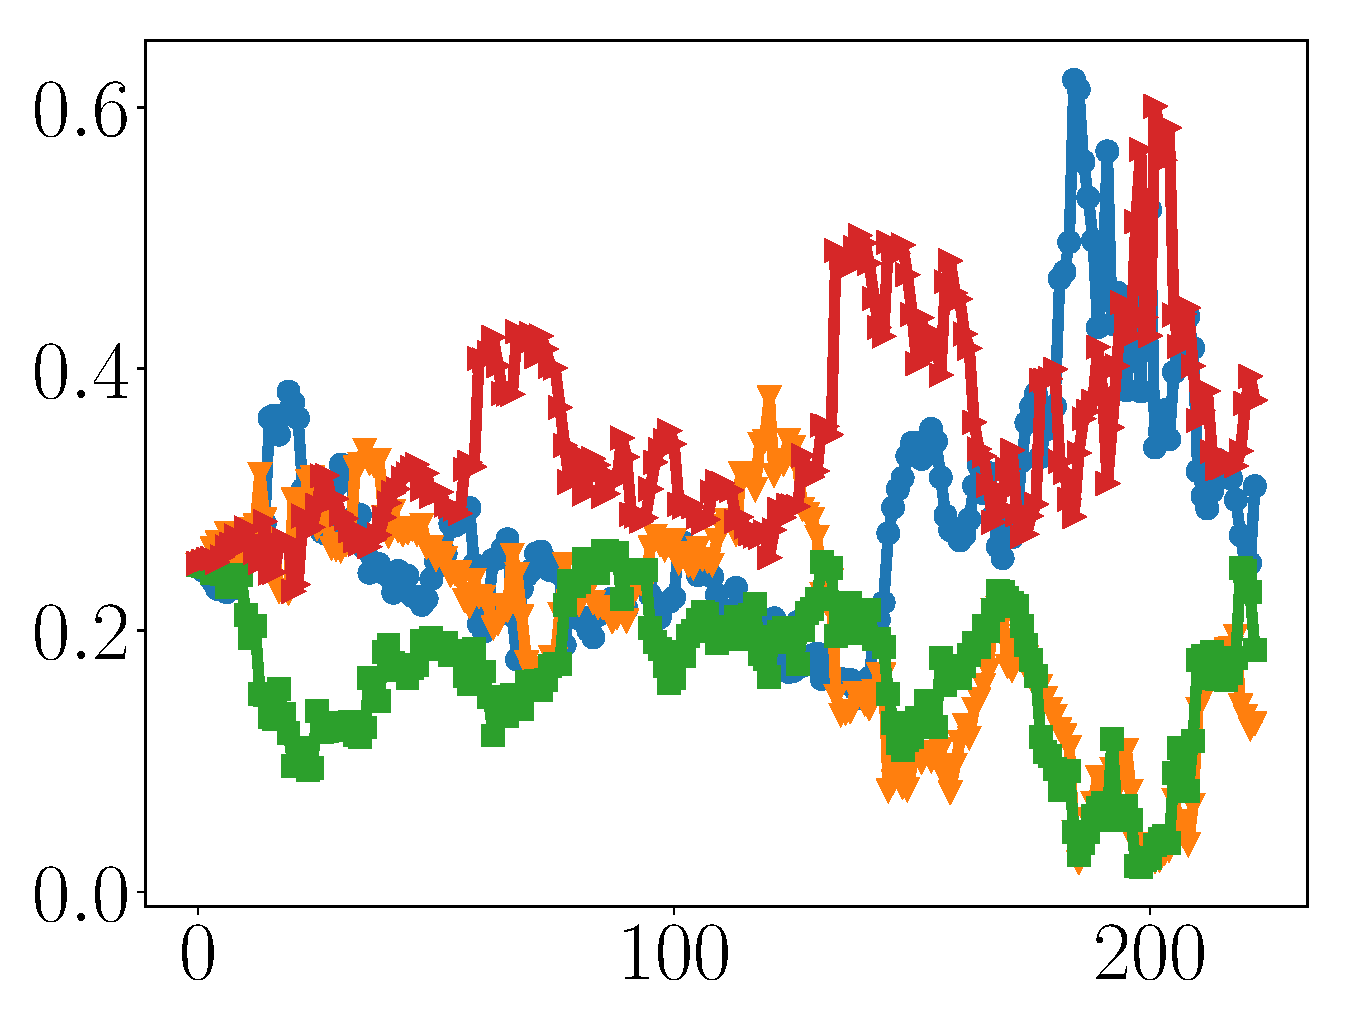
\includegraphics[width=0.22\columnwidth]{figs/aze_uni_probs_plot.eps}
  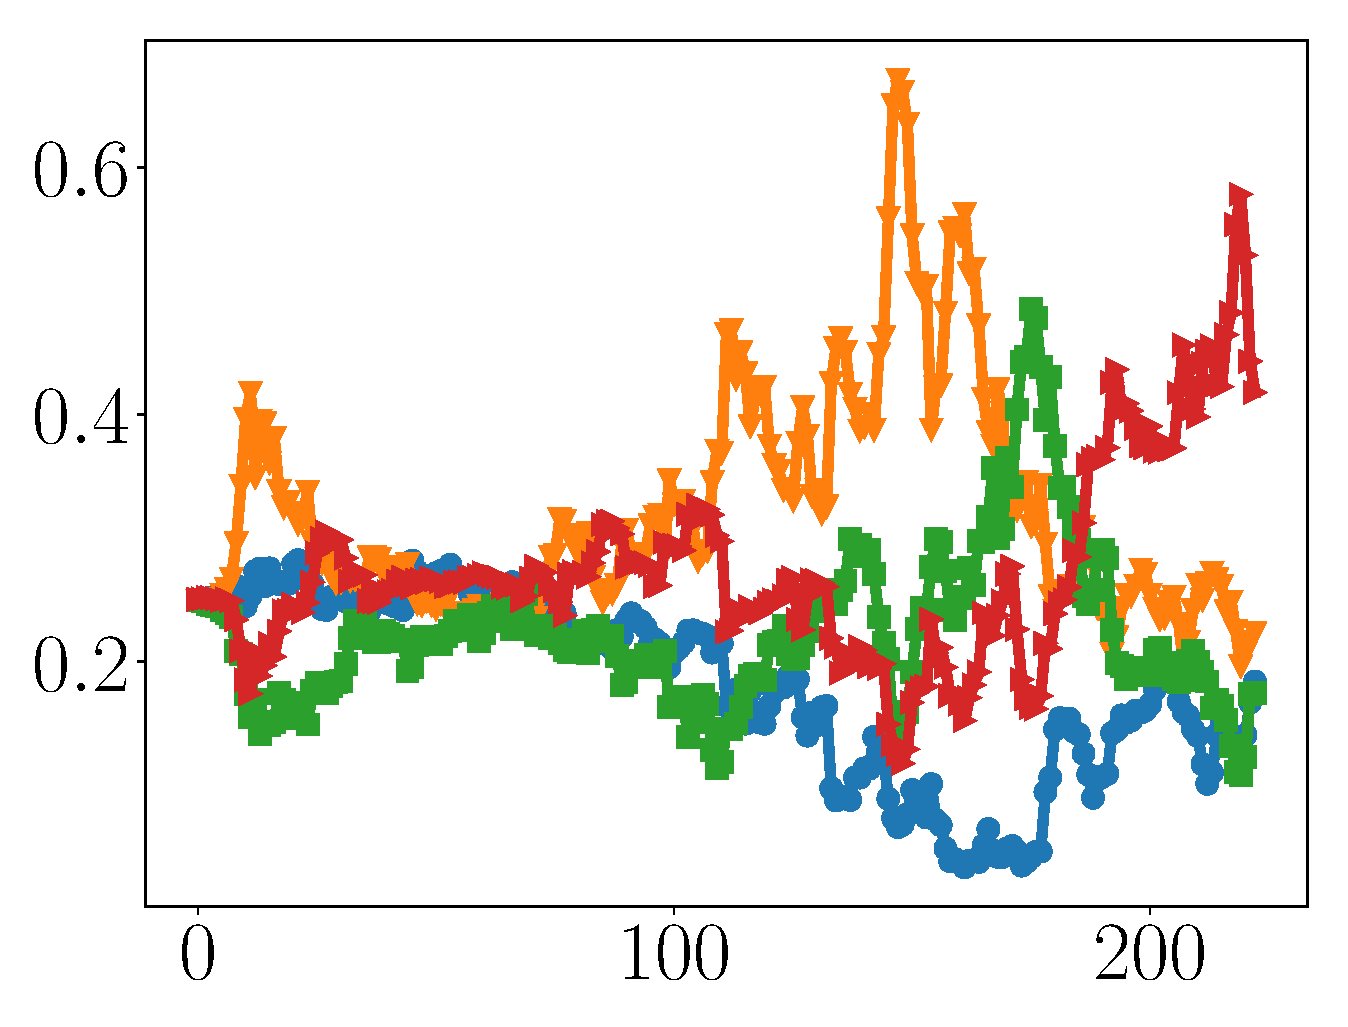
\includegraphics[width=0.22\columnwidth]{figs/bel_uni_probs_plot.eps}
  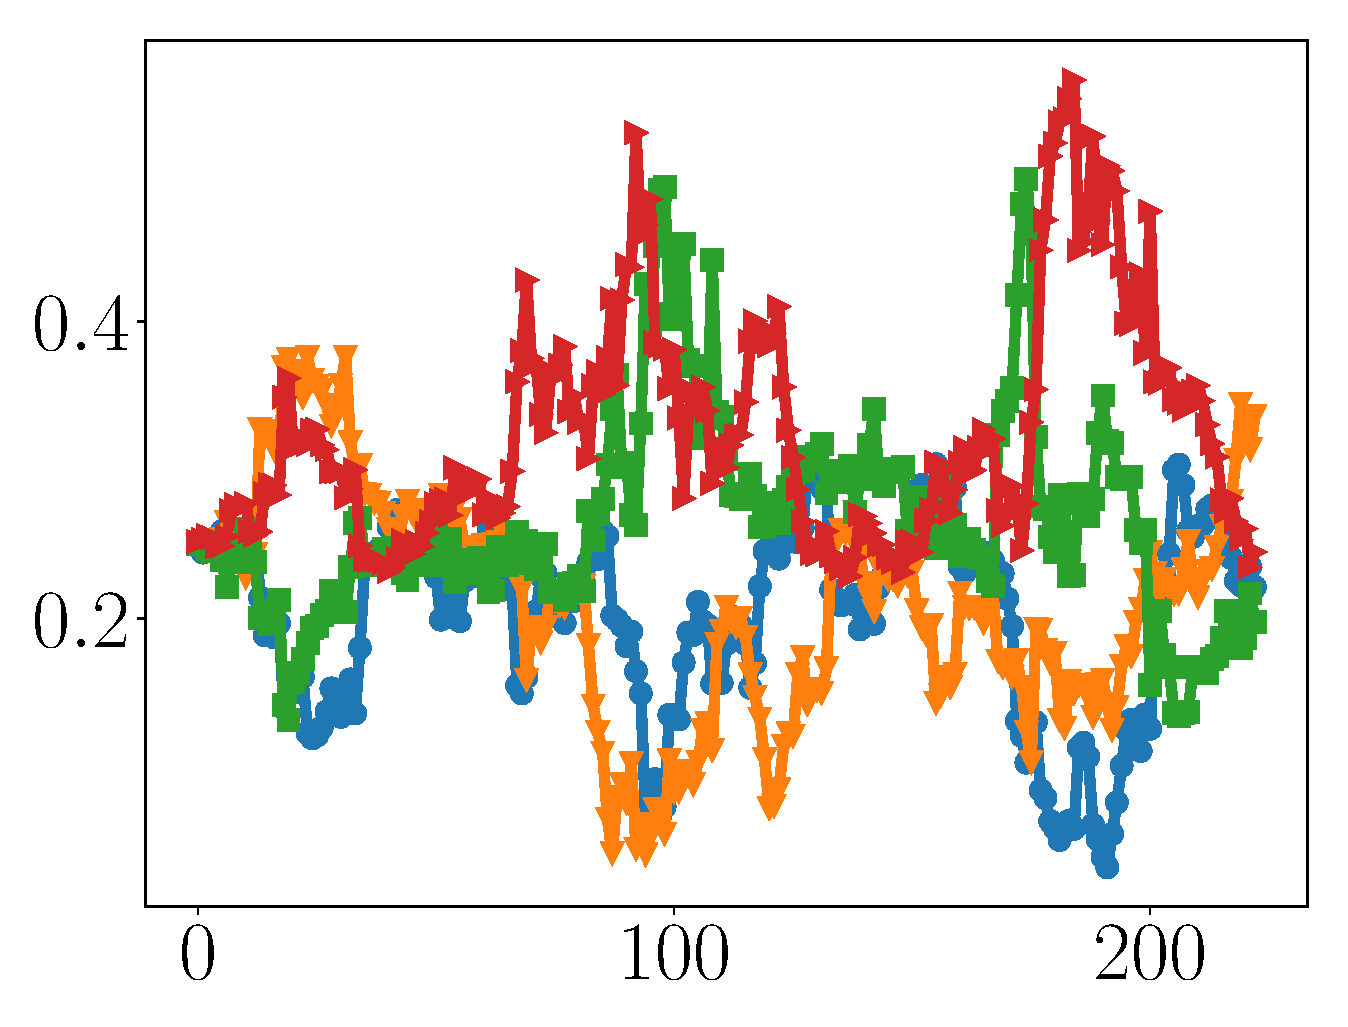
\includegraphics[width=0.22\columnwidth]{figs/glg_uni_probs_plot.eps}
  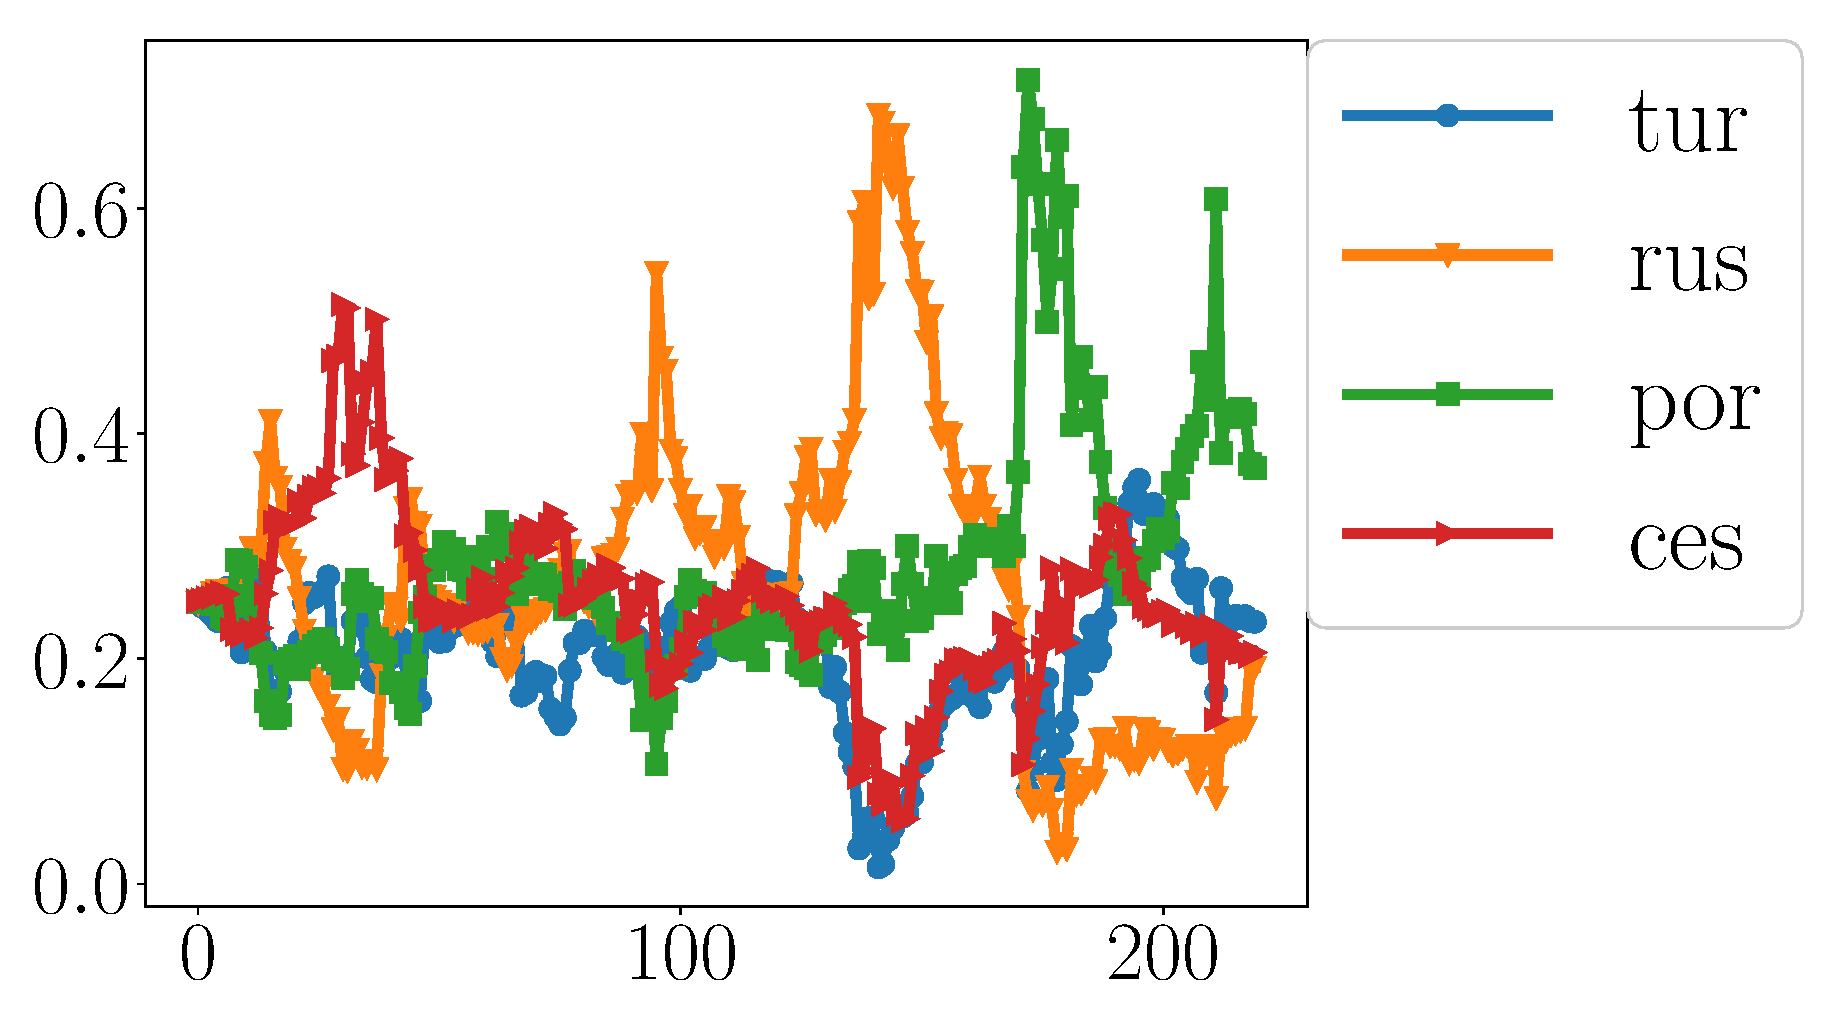
\includegraphics[width=0.29\columnwidth]{figs/slk_uni_probs_plot.eps}
  \captionof{figure}{\label{fig:nmt_distrib_uni}Language usage for DDS by training step. \textit{From left to right}: \texttt{aze}, \texttt{bel}, \texttt{glg}, \texttt{slk}.}
\end{center}
\vspace{-0.2cm}

In Figure \ref{fig:nmt_distrib_uni}, we show a more interesting trend of DDS without heuristic initialization.
For both \texttt{aze} and \texttt{bel}, our method learns to focus on their most related HRL after a certain number of training updates.
Interestingly, for \texttt{bel}, DDS learns to focus on both \texttt{rus}, its most related HRL, and another language \texttt{ces}. Similarly for \texttt{slk}, DDS also learns to focus on \texttt{ces}, its most related HRL, and \texttt{rus}, although there is little vocabulary overlap between \texttt{slk} and \texttt{rus}.
Also notably, the ratios significantly change over the course of training, indicating that different types of data may be more useful during different stages of learning the model.
Notably, DDS shows significant improvements over uniform sampling and other heuristics, demonstrating that it is able to discover when it should use other data, even if the patterns are not immediately intuitive.
%Similar to the trend in Figure \ref{fig:nmt_distrib_hs}, glg tends to use both por, its most related HRL, and ces. 

\section{\label{sec:related_work}Related Works}
%\gn{These are mostly based on stuff for NMT, a broader survey is necessary to increase more general ML methods. I've also only added a small subset of the papers on MT. Please follow the backward and forward references (forward references can be found by clicking the ``cited by'' link in Google Scholar).}

For both NMT and image classification, several prior work has focused on data selection for domain adaptation~\citep{moore2010intelligent,axelrod2011domain,domain_adapt_transfer,jiang-zhai-2007-instance,foster-etal-2010-discriminative,wang-etal-2017-instance}, generally using heuristics to measure domain similarity. \cite{domain_adapt_transfer} propose to estimate the importance weight of the classification labels in the pretraining dataset to mitigate the domain differences, while DDS is a more general data selection framework that works for both classification and other usage cases. Besides domain adaptation, it is also found that selecting good examples from the training data can improve NMT~\citep{vyas-etal-2018-identifying,pham-etal-2018-fixing}.  

The formulation of DDS involves bilevel optimization~\citep{bilevel_optim,hier_optim}, which is utilized in several prior work in areas other than data selection~\citep{darts,hyper_grad,finn2017model}. Notably, \cite{darts} proposes a nested optimization to link training and dev set, similar to the general philosophy behind DDS. \cite{darts} utilizes this formulation for efficient neural architecture search, while DDS is designed for efficient data usage.

More generally, our method is also related to the general machine learning problem of teaching. Firstly, hardness-based teaching in curriculum learning estimate the curriculum based on an heuristic understading of the hardness of data~\citep{cl_bengio,automate_cl_GravesBMMK17,SpitkovskyAJ10,zhang2016boosting,zhang2018empirical,platanios19naacl,baysian_curriculum}. These methods, though effective, are harder to generalize because they often require task-specific features. On the other hand, self-paced learning~\citep{spl_visual_category,spl_kumar,spl_visual_category} defines the hardness of the data based on the loss from the main model. This method requires less heuristic estimates, but is still based on the assumption that easy examples should be learned first. Secondly, the recently proposed learning to teach~\citep{learn_to_teach} is probably closer to our setting, where they train a teacher model so that it can ``teach'' the main model better. However, their method requires featurizing the data and student models so that the teacher model could be trained with reinforcement learning. In comparison, our method focuses on data selection, and provides a much simpler framework without feature engineering. 

%Lastly, our method is related to the work on investigating the effect of label noise on deep image recognition models \cite{rolnick2017deep,overfit_random_examples} or machine translation \cite{khayrallah-koehn-2018-impact}, while \citet{koh2017understanding} shows the feasibility of training set poisoning attacks.


%Instance weighting: \cite{jiang-zhai-2007-instance,foster-etal-2010-discriminative,wang-etal-2017-instance}. In particular, \cite{wang-etal-2017-instance} seems like a good paper to compare against because it's recent and based on neural MT.

%Curriculum learning: \cite{zhang2016boosting,zhang2018empirical,platanios19naacl}.

%Data selection: \cite{moore2010intelligent,axelrod2011domain}.

%Removing bad training examples improves MT: \cite{vyas-etal-2018-identifying,pham-etal-2018-fixing}

%Dataset poisoning (for neural models): \cite{koh2017understanding}



%Meta-learning. Formulation of using the gradient update equation is similar to MAML \cite{finn2017model}.
\section{\label{sec:conclusion}Conclusion}
We present Differentiable Data Selection, an automatic data selection framework for optimizing data usage of deep learning models. Our method does not require domain knowledge for heuristic design, and instead directly optimizes the training data distribution along with the main model. We formulate two algorithms under the DDS framework for both multilingual NMT and image classification, which lead to consistent improvement over strong baselines. 


%\newpage

\bibliography{main}
\bibliographystyle{icml2019}

\newpage
\appendix
\section{\label{app} Appendix}

\subsection{\label{app:grad_of_optimizers}Deriving $\nabla_\psi g$ for Different Optimizers}
%\gn{It seems reasonable to have this as a top-level section, so I changed it accordingly this has started to get into details that are probably better to separate from the overall high-level idea of DDS.}

Here we first derive $\nabla_\psi g$ for the general stochastic gradient descent~(SGD) update, then provide examples for two other common optimization algorithms, namely Momentum~\citep{nesterov} and Adam~\citep{adam}.
%\gn{It's not clear to me why you skip standard SGD without momentum? It seems like it'd make the most sense to start there, even if that's not what you finally use in experiments. If you use it in experiments then you definitely need to discuss it. Then when you explain momentum you could just point out the differences.}

\paragraph{SGD Updates.} The SGD update rule for $\theta$ is as follows
\begin{equation}
  \label{eqn:sgd_update}
   \small
  \begin{aligned}
    \theta_t &\leftarrow \theta_{t-1} - \eta_t \nabla_\theta J(\theta_{t-1}, \psi)
  \end{aligned}
\end{equation}
where $\eta_t$ is the learning rate. Matching the updates in Eqn~\ref{eqn:sgd_update} with the generic framework in Eqn~\ref{eqn:theta_update_rule}, we can see that $g$ in Eqn~\ref{eqn:theta_update_rule} has the form: %\gn{$J(\theta_{t-1})$ should be $J(\theta_{t-1}, \psi)$? There seem to be a few of these inconsistencies below as well, so please check. Also, which time step of $\theta$ does the gradient depend on?}
\begin{equation}
  \label{eqn:momentum_update_g}
   \small
  \begin{aligned}
    g\big(\nabla_\theta J(\theta_{t-1}, \psi)\big) = \eta_t \nabla_\theta J(\theta_{t-1}, \psi)
  \end{aligned}
\end{equation}
This reveals a linear dependency of $g$ on $\nabla_\theta J(\theta_{t-1, \psi})$, allowing the exact differentiation of $g$ with respect to $\psi$. From Eqn~\ref{eqn:psi_update_rule}, we have
\begin{equation}
  \label{eqn:momentum_update_for_psi}
   \small
  \begin{aligned}
    &\nabla J(\theta_t, \mathcal{D}_\text{dev})^\top \cdot \nabla_\psi g\big( \nabla_\theta J(\theta_{t-1}, \psi) \big) \\
    &= \eta_t \cdot \nabla_\psi \mathbb{E}_{x, y \sim p(X, Y; \psi)} \left[J(\theta_t, \mathcal{D}_\text{dev})^\top \cdot \nabla_\theta \ell(x, y; \theta_{t-1} )\right] \\
    &= \eta_t \mathbb{E}_{x, y \sim p(X, Y; \psi)} \left[\left( J(\theta_t, \mathcal{D}_\text{dev})^\top \cdot \nabla_\theta \ell(x, y; \theta_{t-1} ) \right) \cdot \nabla_\psi \log{p(x, y; \psi)} \right]
  \end{aligned}
\end{equation}
%\gn{This last paragraph was too dense for me to follow: could you please try to explain a little more?}
Here, the last equation follows from the log-derivative trick in the REINFORCE algorithm~\citep{reinforce}. 
%and can be implemented by Monte Carlo approximation.
%\gn{again, a little more detail here would be useful}. 
%Note we do not do reinforcement learning in this paper. Instead \gn{this ``instead'' was also not clear to me.}, we simply utilize the same log-derivative trick to compute $\nabla_\psi J(\theta_t, \mathcal{D}_\text{dev})$. 

\paragraph{Momentum Updates.} The momentum update rule for $\theta$ is as follows
\begin{equation}
  \label{eqn:momentum_update}
   \small
  \begin{aligned}
    m_t &\leftarrow \mu_t m_{t-1} + \eta_t \nabla_\theta J(\theta_{t-1}, \psi) \\
    \theta_t &\leftarrow \theta_{t-1} - m_t,
  \end{aligned}
\end{equation}
where $\mu_t$ is the momentum coefficient and $\eta_t$ is the learning rate. This means that $g$ has the form:
\begin{equation}
  \label{eqn:momentum_update_g}
   \small
  \begin{aligned}
    g(x) &= \mu m_{t-1} + \eta_t x \\
    g'(x) &= \eta_t
  \end{aligned}
\end{equation}
Therefore, the computation of the gradient $\nabla_{\psi}$ for the Momentum update is exactly the same with the standard SGD update rule in Eqn \ref{eqn:momentum_update_for_psi}.


\paragraph{Adam Updates.} We use a slightly modified update rule based on Adam~\citep{adam}:
\begin{equation}
  \label{eqn:adam_update}
   \small
  \begin{aligned}
    &g_t \leftarrow \nabla_\theta J(\theta_{t-1}, \psi) \\
    &v_t \leftarrow \beta_2 v_{t-1} + (1 - \beta_2) g_t^2 \\
    &\hat{v}_t \leftarrow v_t / (1 - \beta_2^t) \\
    &\theta_t \leftarrow \theta_{t-1} - \eta_t \cdot g_t / \sqrt{\hat{v}_t + \epsilon}
  \end{aligned}
\end{equation}
where $\beta_2$ and $\eta_t$ are hyper-parameters. This means that $g$ is a component-wise operation of the form:
\begin{equation}
  \label{eqn:adam_update_g}
   \small
  \begin{aligned}
    g(x) &= \frac{\eta_t \sqrt{1 - \beta_2^t} \cdot x}{\sqrt{\beta_2 v_{t-1} + (1 - \beta_2) x^2 + \epsilon}} \\
    g'(x) &= \frac{\eta_t \sqrt{1 - \beta_2^t} (\beta_2 v_{t-1} + \epsilon)}{\big( \beta_2 v_{t-1} + (1 - \beta_2) x^2 + \epsilon \big)^{3/2}} \approx \eta_t \sqrt{\frac{1 - \beta_2^t}{\beta_2 v_{t-1}}},  
  \end{aligned}
\end{equation}
%\paul{So all of this is under the assumption that $v_{t-1}$ is independent on $\psi$ right? maybe bring it up?}
the last equation holds because we assume $v_{t-1}$ is independent of $\psi$. Here the approximation makes sense because we empirically observe that the individual values of the gradient vector $\nabla_\theta J(\theta_{t-1}, \psi)$,~\ie~$g_t$, are close to $0$. Furthermore, for Adam, we usually use $\beta_2 = 0.999$. Thus, the value $(1 - \beta_2) x^2$ in the denominator of Eqn~\ref{eqn:adam_update_g} is negligible. With this approximation, the computation of the gradient $\nabla_\psi$ is almost the same with that for SGD in Eqn~\ref{eqn:momentum_update_for_psi}, with one extra component-wise scaling by the term in Eqn~\ref{eqn:adam_update_g}.

\subsection{\label{app:nmt_hparam} Hyperparameters for multilingual NMT}
In this section, we give a detailed description of the hyperparameters used for the multilingual NMT experiments.
\begin{itemize}
    \item We use a 1 layer LSTM with hidden size of 512 for both the encoder and decoder, and set the word embedding to size 128.
    \item The dropout rate is set to 0.3.
    \item For the NMT model, we use Adam optimizer with learning rate of 0.001. For the distribution parameter $\psi$, we use Adam optimizer with learning rate of 0.0001.
    \item We train all models for 20 epochs without any learning rate decay.
\end{itemize}

\subsection{\label{app:nmt_data} Dataset statistics for Multilingual NMT}
\begin{table}[H]
%\begin{wraptable}{r}{4.3cm}
  \centering
   %\resizebox{0.3\textwidth}{!}{
  \begin{tabular}{c|ccc|cc}
  \toprule
  \textbf{LRL} & \textbf{Train} & \textbf{Dev} & \textbf{Test} & \textbf{HRL} & \textbf{Train} \\
  \midrule
  aze & 5.94k &  671 &  903 & tur & 182k \\
  bel & 4.51k &  248 &  664 & rus & 208k \\
  glg & 10.0k &  682 & 1007 & por & 185k \\
  slk & 61.5k & 2271 & 2445 & ces & 103k \\
  \bottomrule
  \end{tabular}
  %}
  \vspace{0.2cm}
  \caption{\label{tab:nmt_data}Statistics of the multilingual NMT datasets.}
% \end{wraptable}
\end{table} 

\subsection{\label{app:image_hparam} Hyperparameters for image classification}
In this section, we provide some additional details for the image classification task:
\begin{itemize}
  \item We use the cosine learning rate decay schedule~\citep{cosine_lr}, starting at $0.1$ for CIFAR-10 and $3.2$ for ImageNet, both with $2000$ warmup steps. 
  \item We maintain a moving average of all model parameters with the rate of $0.999$. Following~\citet{imagenet_generalize_better}, we treat the moving statistics of batch normalization~\citep{batch_norm} as \textit{untrained parameters} and also add them to the moving averages. 
\end{itemize}

%\subsection{\label{app:image_detail} Training details for image classification}
%Our experiments were conducted on second-generation Tensor Processing Units (TPUv2). There were several important implementation details related to improving training efficiency with DDS for ImageNet models (these were not needed for the smaller CIFAR-10 training set). First, each batch of $4096$ training instances for ImageNet is processed in parallel on $32$ TPU cores, each working on $128$ images. When we compute $p(\hat{x}, \hat{y}; \psi)$ (in~Section \ref{sec:image_method}), the softmax function is computed \textit{locally on each core} to reduce the synchronization overhead. Second, since we do not need the parameters $\psi$ of the DDS model, we ignore all batch normalization moving average updates when we pass images through $p(\hat{x}, \hat{y}; \psi)$. We also only batch-normalize the DDS model locally on each TPU core. Controlled profiling measures show that the aforementioned details speed up the training process by almost $2.5 \times$. Third, following~\citet{neural_combi} and~\citet{enas}, for ImageNet, we apply a $\tanh$ activation to the logits prior to the softmax to compute $p(\hat{x}, \hat{y}; \psi)$, which softens the softmax distribution and prevents the $p(\hat{x}, \hat{y}; \psi)$ from collapsing into always choosing a particular example.

\subsection{Training Time}
For NMT, the baseline TCS takes 10 hours, and DDS takes about 24 hours to finish. Our NMT code is not optimized and can potentially be made much more efficient. 
For CIFAR-10, DDS take about $9$ hours, while experiments without DDS takes $5.5$ hours, and for ImageNet, these take $4$ hours and $6$ hours approximately. 




\end{document}


% This document was modified from the file originally made available by
% Pat Langley and Andrea Danyluk for ICML-2K. This version was created
% by Iain Murray in 2018, and modified by Alexandre Bouchard in
% 2019. Previous contributors include Dan Roy, Lise Getoor and Tobias
% Scheffer, which was slightly modified from the 2010 version by
% Thorsten Joachims & Johannes Fuernkranz, slightly modified from the
% 2009 version by Kiri Wagstaff and Sam Roweis's 2008 version, which is
% slightly modified from Prasad Tadepalli's 2007 version which is a
% lightly changed version of the previous year's version by Andrew
% Moore, which was in turn edited from those of Kristian Kersting and
% Codrina Lauth. Alex Smola contributed to the algorithmic style files.
